\documentclass[a4paper,12pt]{article}

%====================================================
%================== PACOTES (IMPORTS) ===============
%====================================================

% --- Configuração de Página e Idioma ---
\usepackage[papersize={216mm,330mm},tmargin=20mm,bmargin=20mm,lmargin=20mm,rmargin=20mm]{geometry}
\usepackage[brazil]{babel}
\usepackage[utf8]{inputenc}

% --- Pacotes Matemáticos ---
\usepackage{amsmath,amssymb}
\usepackage{amsthm}
\usepackage{mathtools}
\usepackage{cancel}

% --- Layout e Formatação ---
\usepackage{graphicx}
\usepackage{lscape}
\usepackage{fancyhdr}
\usepackage{multicol}
\usepackage{parcolumns}
\usepackage{enumitem}
\usepackage{ragged2e} % Para justificar texto
\usepackage{pdflscape}
\usepackage{color}
\usepackage{colortbl}
\usepackage[utf8]{inputenc}
\usepackage{amsmath}
\usepackage{amsfonts}
\usepackage{amssymb}
\usepackage{graphicx}
\usepackage{array}

% --- Ferramentas e Utilitários ---
\usepackage{float}
\usepackage[colorinlistoftodos]{todonotes}
\usepackage{tasks}
\usepackage{stackengine}
\usepackage{hyperref} % SUGESTÃO: Para links clicáveis na TOC. Geralmente é o último a ser carregado.

% --- Pacotes para Desenho (Gráficos) ---
\usepackage{tikz}
\usepackage{tkz-fct}

% --- Definição de Teoremas ---
% CORREÇÃO: O pacote amsthm estava sendo carregado duas vezes. Agora está apenas uma.
\newtheorem{theorem}{Teorema}

%====================================================
%============= INFORMAÇÕES DE ENTRADA ===============
%====================================================
% CORREÇÃO: Removidos espaços invisíveis (non-breaking spaces) do final das linhas.
\def\nomedoaluno{Caio Daniel Fonseca de Araújo, Arthur Queiroz Pires De Farias, Matheus Rivaldo Da Silva, Paulo Roberto Fernandes Holanda, Marcela Silva Batista}
\def\coddisciplina{DIM0549}
\def\nomedisciplina{Grafos}
\def\codturma{T01 (2025.2)}
\def\codatividade{Trabalho Unidade 01}

%====================================================
%====================== FIM =========================
%====================================================

% --- Configuração do Cabeçalho e Rodapé ---
\pagestyle{fancy}
\fancyhf{}
\lhead{Instituto Metrópole Digital - UFRN}
\chead{\thepage}
\rhead{Turma \codturma}
\lfoot{\nomedisciplina}
\rfoot{Prof. Matheus da Silva Menezes}

% --- Informações do Título ---
% CORREÇÃO: \author{} e \date{} foram removidos do preâmbulo, pois já estão definidos aqui dentro.
\date{\today}
% --- Informações do Título ---
% --- Informações do Título (Estrutura Unificada) ---
\title{
    \vspace{-2.5cm} % Ajuste fino para subir o bloco na página
    \centering % Centraliza todo o conteúdo do título
    \Large\textbf{Universidade Federal do Rio Grande do Norte}\\
    \large Instituto Metrópole Digital \\[0.5em]
    \normalsize \coddisciplina{} -- \nomedisciplina{} -- Turma \codturma \\[1.5em]
    \Large\textbf{\codatividade} \\[1.5em]
    \large\textbf{Colaboradores} \\
    \normalsize\textit{\nomedoaluno} \\[1em]
    \large\textbf{Professor} \\
    \normalsize\textit{Prof. Matheus da Silva Menezes} \\[2.5em]
    \normalsize Natal-RN, \today
    \vspace{-0.5cm} % Espaço antes do corpo do documento
}
% Deixe os comandos \author{} e \date{} vazios no preâmbulo
\author{}
\date{}

\setlength{\marginparwidth}{2cm}

%====================================================
%================ INÍCIO DO DOCUMENTO ===============
%====================================================

\begin{document}
\maketitle

\section*{\centering Apresentação}
Este documento apresenta os resultados obtidos através da biblioteca em Python desenvolvida para a disciplina de Grafos. Foram analisados 8 arquivos, contendo representações de grafos não-direcionados e dígrafos. Para cada um, foram aplicadas as funcionalidades implementadas, conforme detalhado nas seções a seguir.

\subsection*{Sumário}
\tableofcontents
\newpage

% =====================================================================
% =================== SEÇÃO PARA GRAFOS ===============================
% =====================================================================
\section{Análise dos Grafos Não-Direcionados}

% ----------------- GRAFO_0.txt -----------------
\subsection{Resultados para o arquivo: GRAFO\_0.txt}

\begin{center}
    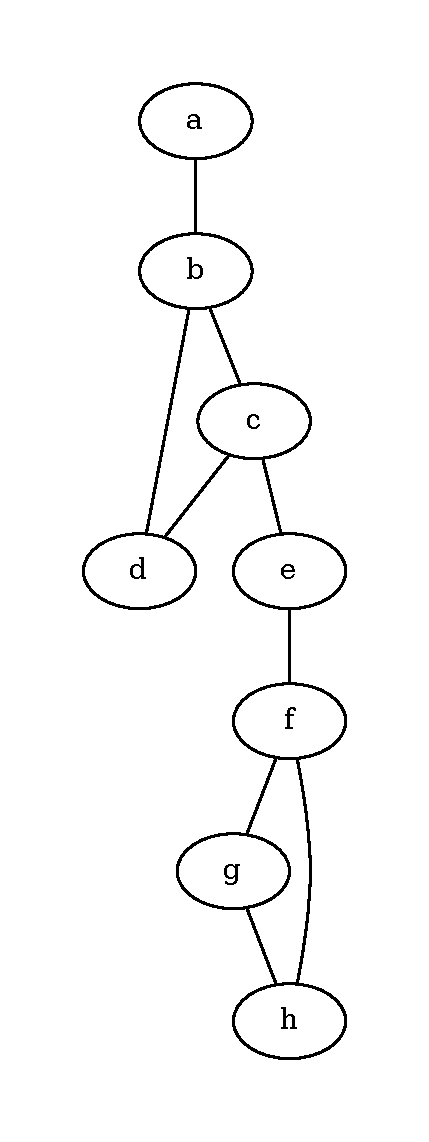
\includegraphics[width=0.4\textwidth]{imagens/render/GRAFO_0.png}
\end{center}

\subsubsection*{Atividade A.1: Criação a partir da Lista de Adjacências}
A estrutura do grafo é definida pela seguinte lista de adjacências:
\begin{itemize}[leftmargin=*]
    \item[\textbf{a:}] ['b']
    \item[\textbf{b:}] ['a', 'c', 'd']
    \item[\textbf{c:}] ['b', 'd', 'e']
    \item[\textbf{d:}] ['b', 'c']
    \item[\textbf{e:}] ['c', 'f']
    \item[\textbf{f:}] ['e', 'g', 'h']
    \item[\textbf{g:}] ['f', 'h']
    \item[\textbf{h:}] ['f', 'g']
\end{itemize}

\subsubsection*{Atividade A.2: Criação a partir da Matriz de Adjacências}
A estrutura do grafo é definida pela seguinte matriz de adjacências:
\begin{center}
\scriptsize
\begin{tabular*}{\textwidth}{c|@{\extracolsep{\fill}}cccccccc}
\rowcolor[gray]{0.9}
 & \textbf{a} & \textbf{b} & \textbf{c} & \textbf{d} & \textbf{e} & \textbf{f} & \textbf{g} & \textbf{h} \\
\hline
\textbf{a} & 0 & 1 & 0 & 0 & 0 & 0 & 0 & 0 \\
\textbf{b} & 1 & 0 & 1 & 1 & 0 & 0 & 0 & 0 \\
\textbf{c} & 0 & 1 & 0 & 1 & 1 & 0 & 0 & 0 \\
\textbf{d} & 0 & 1 & 1 & 0 & 0 & 0 & 0 & 0 \\
\textbf{e} & 0 & 0 & 1 & 0 & 0 & 1 & 0 & 0 \\
\textbf{f} & 0 & 0 & 0 & 0 & 1 & 0 & 1 & 1 \\
\textbf{g} & 0 & 0 & 0 & 0 & 0 & 1 & 0 & 1 \\
\textbf{h} & 0 & 0 & 0 & 0 & 0 & 1 & 1 & 0 \\
\end{tabular*}
\end{center}

\subsubsection*{Atividade A.3: Criação a partir da Matriz de Incidência}
A matriz de incidência para o grafo (não fornecida, mas gerada a partir dos dados) mapeia vértices (linhas) a arestas (colunas). Para grafos não-direcionados, o valor é \textbf{1} se o vértice pertence à aresta. O grafo possui 9 arestas:
\begin{multicols}{2}
\begin{itemize}[nosep, leftmargin=*]
    \item[$e_1$:] (a,b) \quad \item[$e_2$:] (b,c) \quad \item[$e_3$:] (b,d)
    \item[$e_4$:] (c,d) \quad \item[$e_5$:] (c,e) \quad \item[$e_6$:] (e,f)
    \item[$e_7$:] (f,g) \quad \item[$e_8$:] (f,h) \quad \item[$e_9$:] (g,h)
\end{itemize}
\end{multicols}
\begin{center}
\scriptsize
\begin{tabular*}{\textwidth}{c|@{\extracolsep{\fill}}ccccccccc}
\rowcolor[gray]{0.9}
 & \textbf{$e_1$} & \textbf{$e_2$} & \textbf{$e_3$} & \textbf{$e_4$} & \textbf{$e_5$} & \textbf{$e_6$} & \textbf{$e_7$} & \textbf{$e_8$} & \textbf{$e_9$} \\
\hline
\textbf{a} & 1 & 0 & 0 & 0 & 0 & 0 & 0 & 0 & 0 \\
\textbf{b} & 1 & 1 & 1 & 0 & 0 & 0 & 0 & 0 & 0 \\
\textbf{c} & 0 & 1 & 0 & 1 & 1 & 0 & 0 & 0 & 0 \\
\textbf{d} & 0 & 0 & 1 & 1 & 0 & 0 & 0 & 0 & 0 \\
\textbf{e} & 0 & 0 & 0 & 0 & 1 & 1 & 0 & 0 & 0 \\
\textbf{f} & 0 & 0 & 0 & 0 & 0 & 1 & 1 & 1 & 0 \\
\textbf{g} & 0 & 0 & 0 & 0 & 0 & 0 & 1 & 0 & 1 \\
\textbf{h} & 0 & 0 & 0 & 0 & 0 & 0 & 0 & 1 & 1 \\
\end{tabular*}
\end{center}

\subsubsection*{Atividade A.4: Conversão de Representações}
\paragraph*{Matriz de Adjacências $\rightarrow$ Lista de Adjacências:}
\begin{itemize}[leftmargin=*]
    \item[\textbf{a:}] ['b'] \item[\textbf{b:}] ['a', 'c', 'd'] \item[\textbf{c:}] ['b', 'd', 'e'] \item[\textbf{d:}] ['b', 'c']
    \item[\textbf{e:}] ['c', 'f'] \item[\textbf{f:}] ['e', 'g', 'h'] \item[\textbf{g:}] ['f', 'h'] \item[\textbf{h:}] ['f', 'g']
\end{itemize}

\paragraph*{Lista de Adjacências $\rightarrow$ Matriz de Adjacências:}
\begin{center}
\scriptsize
\begin{tabular*}{\textwidth}{c|@{\extracolsep{\fill}}cccccccc}
\rowcolor[gray]{0.9}
 & \textbf{a} & \textbf{b} & \textbf{c} & \textbf{d} & \textbf{e} & \textbf{f} & \textbf{g} & \textbf{h} \\ \hline
\textbf{a} & 0 & 1 & 0 & 0 & 0 & 0 & 0 & 0 \\ \textbf{b} & 1 & 0 & 1 & 1 & 0 & 0 & 0 & 0 \\
\textbf{c} & 0 & 1 & 0 & 1 & 1 & 0 & 0 & 0 \\ \textbf{d} & 0 & 1 & 1 & 0 & 0 & 0 & 0 & 0 \\
\textbf{e} & 0 & 0 & 1 & 0 & 0 & 1 & 0 & 0 \\ \textbf{f} & 0 & 0 & 0 & 0 & 1 & 0 & 1 & 1 \\
\textbf{g} & 0 & 0 & 0 & 0 & 0 & 1 & 0 & 1 \\ \textbf{h} & 0 & 0 & 0 & 0 & 0 & 1 & 1 & 0 \\
\end{tabular*}
\end{center}

\subsubsection*{Atividade A.5: Cálculo do Grau dos Vértices}
\begin{multicols}{3}
\begin{itemize}[nosep]
    \item $d(a) = 1$ \item $d(b) = 3$ \item $d(c) = 3$
    \item $d(d) = 2$ \item $d(e) = 2$ \item $d(f) = 3$
    \item $d(g) = 2$ \item $d(h) = 2$
\end{itemize}
\end{multicols}

\subsubsection*{Atividade A.6: Adjacência entre Vértices}
% As opções alinham o rótulo à esquerda, sem recuo da margem principal.
\begin{itemize}[align=left, leftmargin=40pt, labelsep=1em]
    \item[Adjacentes de a:] ['b']
    \item[Adjacentes de b:] ['a', 'c', 'd']
    \item[Adjacentes de c:] ['b', 'd', 'e']
    \item[Adjacentes de d:] ['b', 'c']
    \item[Adjacentes de e:] ['c', 'f']
    \item[Adjacentes de f:] ['e', 'g', 'h']
    \item[Adjacentes de g:] ['f', 'h']
    \item[Adjacentes de h:] ['f', 'g']
\end{itemize}

\subsubsection*{Atividade A.7: Número Total de Vértices}
O grafo possui \textbf{8} vértices: \{a, b, c, d, e, f, g, h\}.

\subsubsection*{Atividade A.8: Número Total de Arestas}
O grafo possui \textbf{9} arestas.

\subsubsection*{Atividade A.9: Inclusão de Vértice}
\textit{Esta operação não foi demonstrada no arquivo de análise.}

\subsubsection*{Atividade A.10: Exclusão de Vértice}
\textit{Esta operação não foi demonstrada no arquivo de análise.}

\subsubsection*{Atividade A.11: Verificação de Conectividade}
O grafo é \textbf{conexo}.

\subsubsection*{Atividade A.12: Verificação de Bipartição}
O grafo \textbf{não} é bipartido.

\subsubsection*{Atividade A.13: Busca em Largura (BFS)}
\begin{center}
    \includegraphics[width=0.3\textwidth]{imagens/render/bfs/GRAFO_0_BFS.png}
\end{center}

\subsubsection*{Atividade A.14: Busca em Profundidade (DFS)}
\begin{center}
    \includegraphics[width=0.3\textwidth]{imagens/render/dfs/GRAFO_0_DFS.png}
\end{center}

\subsubsection*{Atividade A.15: Determinação de Articulações e Blocos}
\begin{itemize}[nosep, leftmargin=*]
    \item \textbf{Pontos de Articulação (Vértices de Corte):} ['b', 'c', 'e', 'f']
    \item \textbf{Pontes:} [('a', 'b'), ('c', 'e'), ('e', 'f')]
\end{itemize}

\\ \\

% ----------------- GRAFO_1.txt -----------------
\subsection{Resultados para o arquivo: GRAFO\_1.txt}

\begin{center}
    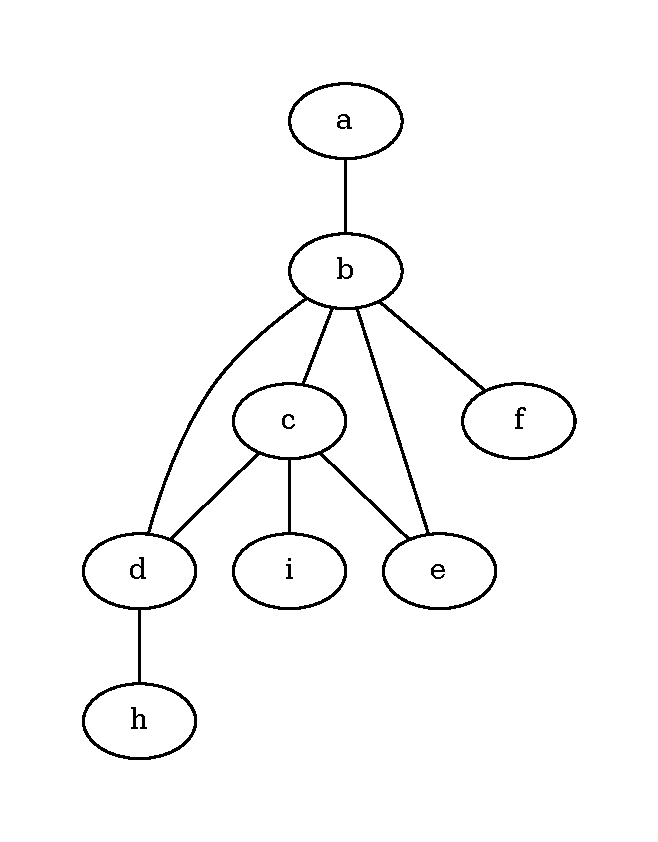
\includegraphics[width=0.6\textwidth]{imagens/render/GRAFO_1.png}
\end{center}

\subsubsection*{Atividade A.1: Criação a partir da Lista de Adjacências}
A estrutura do grafo é definida pela seguinte lista de adjacências:
\begin{itemize}[leftmargin=*]
    \item[\textbf{a:}] ['b']
    \item[\textbf{b:}] ['a', 'c', 'd', 'e', 'f']
    \item[\textbf{c:}] ['b', 'd', 'e', 'i']
    \item[\textbf{d:}] ['b', 'c', 'h']
    \item[\textbf{e:}] ['b', 'c']
    \item[\textbf{f:}] ['b']
    \item[\textbf{h:}] ['d']
    \item[\textbf{i:}] ['c']
\end{itemize}

\subsubsection*{Atividade A.2: Criação a partir da Matriz de Adjacências}
A estrutura do grafo é definida pela seguinte matriz de adjacências:
\begin{center}
\scriptsize
\begin{tabular*}{\textwidth}{c|@{\extracolsep{\fill}}cccccccc}
\rowcolor[gray]{0.9}
 & \textbf{a} & \textbf{b} & \textbf{c} & \textbf{d} & \textbf{e} & \textbf{f} & \textbf{i} & \textbf{h} \\
\hline
\textbf{a} & 0 & 1 & 0 & 0 & 0 & 0 & 0 & 0 \\
\textbf{b} & 1 & 0 & 1 & 1 & 1 & 1 & 0 & 0 \\
\textbf{c} & 0 & 1 & 0 & 1 & 1 & 0 & 1 & 0 \\
\textbf{d} & 0 & 1 & 1 & 0 & 0 & 0 & 0 & 1 \\
\textbf{e} & 0 & 1 & 1 & 0 & 0 & 0 & 0 & 0 \\
\textbf{f} & 0 & 1 & 0 & 0 & 0 & 0 & 0 & 0 \\
\textbf{i} & 0 & 0 & 1 & 0 & 0 & 0 & 0 & 0 \\
\textbf{h} & 0 & 0 & 0 & 1 & 0 & 0 & 0 & 0 \\
\end{tabular*}
\end{center}

\subsubsection*{Atividade A.3: Criação a partir da Matriz de Incidência}
A matriz de incidência para o grafo (gerada a partir dos dados) mapeia vértices (linhas) a arestas (colunas). O grafo possui 9 arestas:
\begin{multicols}{2}
\begin{itemize}[nosep, leftmargin=*]
    \item[$e_1$:] (a,b) \quad \item[$e_2$:] (b,c) \quad \item[$e_3$:] (b,d)
    \item[$e_4$:] (b,e) \quad \item[$e_5$:] (b,f) \quad \item[$e_6$:] (c,d)
    \item[$e_7$:] (c,e) \quad \item[$e_8$:] (c,i) \quad \item[$e_9$:] (d,h)
\end{itemize}
\end{multicols}
\begin{center}
\scriptsize
\begin{tabular*}{\textwidth}{c|@{\extracolsep{\fill}}ccccccccc}
\rowcolor[gray]{0.9}
 & \textbf{$e_1$} & \textbf{$e_2$} & \textbf{$e_3$} & \textbf{$e_4$} & \textbf{$e_5$} & \textbf{$e_6$} & \textbf{$e_7$} & \textbf{$e_8$} & \textbf{$e_9$} \\
\hline
\textbf{a} & 1 & 0 & 0 & 0 & 0 & 0 & 0 & 0 & 0 \\
\textbf{b} & 1 & 1 & 1 & 1 & 1 & 0 & 0 & 0 & 0 \\
\textbf{c} & 0 & 1 & 0 & 0 & 0 & 1 & 1 & 1 & 0 \\
\textbf{d} & 0 & 0 & 1 & 0 & 0 & 1 & 0 & 0 & 1 \\
\textbf{e} & 0 & 0 & 0 & 1 & 0 & 0 & 1 & 0 & 0 \\
\textbf{f} & 0 & 0 & 0 & 0 & 1 & 0 & 0 & 0 & 0 \\
\textbf{i} & 0 & 0 & 0 & 0 & 0 & 0 & 0 & 1 & 0 \\
\textbf{h} & 0 & 0 & 0 & 0 & 0 & 0 & 0 & 0 & 1 \\
\end{tabular*}
\end{center}

\subsubsection*{Atividade A.4: Conversão de Representações}
\paragraph*{Matriz de Adjacências $\rightarrow$ Lista de Adjacências:}
\begin{itemize}[leftmargin=*]
    \item[\textbf{a:}] ['b'] \item[\textbf{b:}] ['a', 'c', 'd', 'e', 'f'] \item[\textbf{c:}] ['b', 'd', 'e', 'i']
    \item[\textbf{d:}] ['b', 'c', 'h'] \item[\textbf{e:}] ['b', 'c'] \item[\textbf{f:}] ['b']
    \item[\textbf{h:}] ['d'] \item[\textbf{i:}] ['c']
\end{itemize}
\paragraph*{Lista de Adjacências $\rightarrow$ Matriz de Adjacências:}
\begin{center}
\scriptsize
\begin{tabular*}{\textwidth}{c|@{\extracolsep{\fill}}cccccccc}
\rowcolor[gray]{0.9}
 & \textbf{a} & \textbf{b} & \textbf{c} & \textbf{d} & \textbf{e} & \textbf{f} & \textbf{i} & \textbf{h} \\ \hline
\textbf{a} & 0 & 1 & 0 & 0 & 0 & 0 & 0 & 0 \\ \textbf{b} & 1 & 0 & 1 & 1 & 1 & 1 & 0 & 0 \\
\textbf{c} & 0 & 1 & 0 & 1 & 1 & 0 & 1 & 0 \\ \textbf{d} & 0 & 1 & 1 & 0 & 0 & 0 & 0 & 1 \\
\textbf{e} & 0 & 1 & 1 & 0 & 0 & 0 & 0 & 0 \\ \textbf{f} & 0 & 1 & 0 & 0 & 0 & 0 & 0 & 0 \\
\textbf{i} & 0 & 0 & 1 & 0 & 0 & 0 & 0 & 0 \\ \textbf{h} & 0 & 0 & 0 & 1 & 0 & 0 & 0 & 0 \\
\end{tabular*}
\end{center}

\subsubsection*{Atividade A.5: Cálculo do Grau dos Vértices}
\begin{multicols}{3}
\begin{itemize}[nosep]
    \item $d(a) = 1$ \item $d(b) = 5$ \item $d(c) = 4$
    \item $d(d) = 3$ \item $d(e) = 2$ \item $d(f) = 1$
    \item $d(h) = 1$ \item $d(i) = 1$
\end{itemize}
\end{multicols}

\subsubsection*{Atividade A.6: Adjacência entre Vértices}
\begin{itemize}[align=left, leftmargin=40pt, labelsep=1em]
    \item[Adjacentes de a:] ['b']
    \item[Adjacentes de b:] ['a', 'c', 'd', 'e', 'f']
    \item[Adjacentes de c:] ['b', 'd', 'e', 'i']
    \item[Adjacentes de d:] ['b', 'c', 'h']
    \item[Adjacentes de e:] ['b', 'c']
    \item[Adjacentes de f:] ['b']
    \item[Adjacentes de h:] ['d']
    \item[Adjacentes de i:] ['c']
\end{itemize}

\subsubsection*{Atividade A.7: Número Total de Vértices}
O grafo possui \textbf{8} vértices: \{a, b, c, d, e, f, h, i\}.

\subsubsection*{Atividade A.8: Número Total de Arestas}
O grafo possui \textbf{9} arestas.

\subsubsection*{Atividade A.9: Inclusão de Vértice}
\textit{Esta operação não foi demonstrada no arquivo de análise.}

\subsubsection*{Atividade A.10: Exclusão de Vértice}
\textit{Esta operação não foi demonstrada no arquivo de análise.}

\subsubsection*{Atividade A.11: Verificação de Conectividade}
O grafo é \textbf{conexo}.

\subsubsection*{Atividade A.12: Verificação de Bipartição}
O grafo \textbf{não} é bipartido.

\subsubsection*{Atividade A.13: Busca em Largura (BFS)}
\begin{center}
    \includegraphics[width=0.5\textwidth]{imagens/render/bfs/GRAFO_1_BFS.png}
\end{center}

\subsubsection*{Atividade A.14: Busca em Profundidade (DFS)}
\begin{center}
    \includegraphics[width=0.8\textwidth]{imagens/render/dfs/GRAFO_1_DFS.png}
\end{center}

\subsubsection*{Atividade A.15: Determinação de Articulações e Blocos}
\begin{itemize}[nosep, leftmargin=*]
    \item \textbf{Pontos de Articulação (Vértices de Corte):} ['b', 'c', 'd']
    \item \textbf{Pontes:} [('a', 'b'), ('b', 'f'), ('c', 'i'), ('d', 'h')]
\end{itemize}

\\ 

% ----------------- GRAFO_2.txt -----------------
\subsection{Resultados para o arquivo: GRAFO\_2.txt}

\begin{center}
    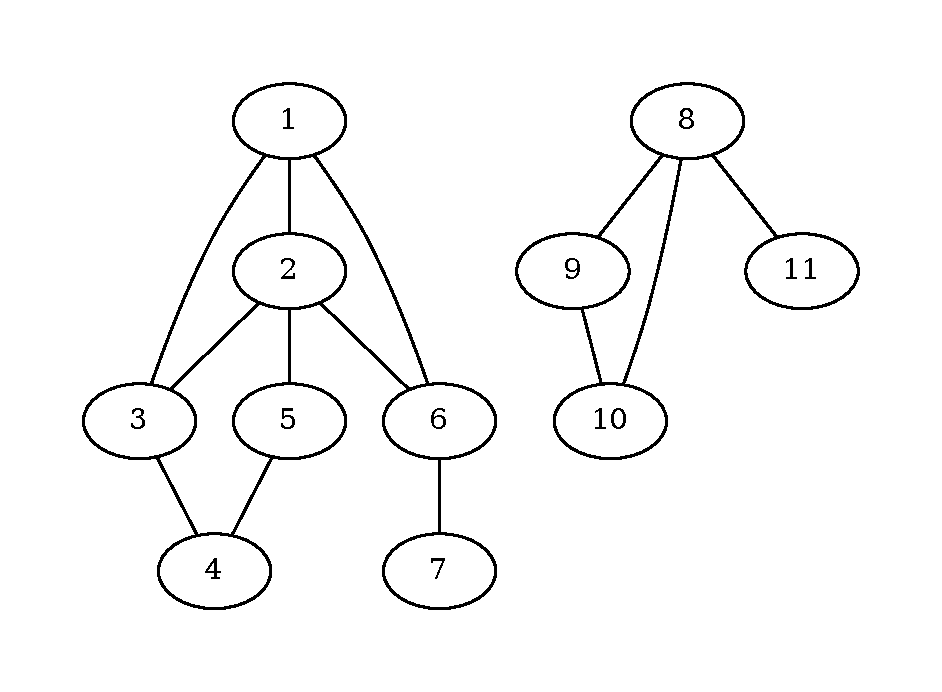
\includegraphics[width=0.6\textwidth]{imagens/render/GRAFO_2.png}
\end{center}

\subsubsection*{Atividade A.1: Criação a partir da Lista de Adjacências}
A estrutura do grafo é definida pela seguinte lista de adjacências:
\begin{itemize}[leftmargin=*]
    \item[\textbf{1:}] ['2', '3', '6']
    \item[\textbf{2:}] ['1', '3', '5', '6']
    \item[\textbf{3:}] ['1', '2', '4']
    \item[\textbf{4:}] ['3', '5']
    \item[\textbf{5:}] ['2', '4']
    \item[\textbf{6:}] ['1', '2', '7']
    \item[\textbf{7:}] ['6']
    \item[\textbf{8:}] ['9', '10', '11']
    \item[\textbf{9:}] ['8', '10']
    \item[\textbf{10:}] ['8', '9']
    \item[\textbf{11:}] ['8']
\end{itemize}

\subsubsection*{Atividade A.2: Criação a partir da Matriz de Adjacências}
A estrutura do grafo é definida pela seguinte matriz de adjacências:
\begin{center}
\scriptsize
\begin{tabular*}{\textwidth}{c|@{\extracolsep{\fill}}ccccccccccc}
\rowcolor[gray]{0.9}
 & \textbf{1} & \textbf{2} & \textbf{3} & \textbf{5} & \textbf{6} & \textbf{4} & \textbf{7} & \textbf{8} & \textbf{9} & \textbf{10} & \textbf{11} \\
\hline
\textbf{1} & 0 & 1 & 1 & 0 & 1 & 0 & 0 & 0 & 0 & 0 & 0 \\
\textbf{2} & 1 & 0 & 1 & 1 & 1 & 0 & 0 & 0 & 0 & 0 & 0 \\
\textbf{3} & 1 & 1 & 0 & 0 & 0 & 1 & 0 & 0 & 0 & 0 & 0 \\
\textbf{5} & 0 & 1 & 0 & 0 & 0 & 1 & 0 & 0 & 0 & 0 & 0 \\
\textbf{6} & 1 & 1 & 0 & 0 & 0 & 0 & 1 & 0 & 0 & 0 & 0 \\
\textbf{4} & 0 & 0 & 1 & 1 & 0 & 0 & 0 & 0 & 0 & 0 & 0 \\
\textbf{7} & 0 & 0 & 0 & 0 & 1 & 0 & 0 & 0 & 0 & 0 & 0 \\
\textbf{8} & 0 & 0 & 0 & 0 & 0 & 0 & 0 & 0 & 1 & 1 & 1 \\
\textbf{9} & 0 & 0 & 0 & 0 & 0 & 0 & 0 & 1 & 0 & 1 & 0 \\
\textbf{10} & 0 & 0 & 0 & 0 & 0 & 0 & 0 & 1 & 1 & 0 & 0 \\
\textbf{11} & 0 & 0 & 0 & 0 & 0 & 0 & 0 & 1 & 0 & 0 & 0 \\
\end{tabular*}
\end{center}

\subsubsection*{Atividade A.3: Criação a partir da Matriz de Incidência}
A matriz de incidência para o grafo (gerada a partir dos dados) mapeia vértices (linhas) a arestas (colunas). O grafo possui 13 arestas:
\begin{multicols}{2}
\begin{itemize}[nosep, leftmargin=*]
    \item[$e_1$:] (1,2) \quad \item[$e_2$:] (1,3) \quad \item[$e_3$:] (1,6)
    \item[$e_4$:] (2,3) \quad \item[$e_5$:] (2,5) \quad \item[$e_6$:] (2,6)
    \item[$e_7$:] (3,4) \quad \item[$e_8$:] (4,5) \quad \item[$e_9$:] (6,7)
    \item[$e_{10}$:] (8,9) \quad \item[$e_{11}$:] (8,10) \quad \item[$e_{12}$:] (8,11)
    \item[$e_{13}$:] (9,10)
\end{itemize}
\end{multicols}
\begin{center}
\scriptsize
\begin{tabular*}{\textwidth}{c|@{\extracolsep{\fill}}ccccccccccccc}
\rowcolor[gray]{0.9}
 & \textbf{$e_1$} & \textbf{$e_2$} & \textbf{$e_3$} & \textbf{$e_4$} & \textbf{$e_5$} & \textbf{$e_6$} & \textbf{$e_7$} & \textbf{$e_8$} & \textbf{$e_9$} & \textbf{$e_{10}$} & \textbf{$e_{11}$} & \textbf{$e_{12}$} & \textbf{$e_{13}$} \\
\hline
\textbf{1} & 1 & 1 & 1 & 0 & 0 & 0 & 0 & 0 & 0 & 0 & 0 & 0 & 0 \\
\textbf{2} & 1 & 0 & 0 & 1 & 1 & 1 & 0 & 0 & 0 & 0 & 0 & 0 & 0 \\
\textbf{3} & 0 & 1 & 0 & 1 & 0 & 0 & 1 & 0 & 0 & 0 & 0 & 0 & 0 \\
\textbf{4} & 0 & 0 & 0 & 0 & 0 & 0 & 1 & 1 & 0 & 0 & 0 & 0 & 0 \\
\textbf{5} & 0 & 0 & 0 & 0 & 1 & 0 & 0 & 1 & 0 & 0 & 0 & 0 & 0 \\
\textbf{6} & 0 & 0 & 1 & 0 & 0 & 1 & 0 & 0 & 1 & 0 & 0 & 0 & 0 \\
\textbf{7} & 0 & 0 & 0 & 0 & 0 & 0 & 0 & 0 & 1 & 0 & 0 & 0 & 0 \\
\textbf{8} & 0 & 0 & 0 & 0 & 0 & 0 & 0 & 0 & 0 & 1 & 1 & 1 & 0 \\
\textbf{9} & 0 & 0 & 0 & 0 & 0 & 0 & 0 & 0 & 0 & 1 & 0 & 0 & 1 \\
\textbf{10} & 0 & 0 & 0 & 0 & 0 & 0 & 0 & 0 & 0 & 0 & 1 & 0 & 1 \\
\textbf{11} & 0 & 0 & 0 & 0 & 0 & 0 & 0 & 0 & 0 & 0 & 0 & 1 & 0 \\
\end{tabular*}
\end{center}

\subsubsection*{Atividade A.4: Conversão de Representações}
\paragraph*{Matriz de Adjacências $\rightarrow$ Lista de Adjacências:}
\begin{itemize}[leftmargin=*]
    \item[\textbf{1:}] ['2', '3', '6'] \item[\textbf{2:}] ['1', '3', '5', '6'] \item[\textbf{3:}] ['1', '2', '4'] \item[\textbf{4:}] ['3', '5']
    \item[\textbf{5:}] ['2', '4'] \item[\textbf{6:}] ['1', '2', '7'] \item[\textbf{7:}] ['6'] \item[\textbf{8:}] ['9', '10', '11']
    \item[\textbf{9:}] ['8', '10'] \item[\textbf{10:}] ['8', '9'] \item[\textbf{11:}] ['8']
\end{itemize}
\paragraph*{Lista de Adjacências $\rightarrow$ Matriz de Adjacências:}
\begin{center}
\scriptsize
\begin{tabular*}{\textwidth}{c|@{\extracolsep{\fill}}ccccccccccc}
\rowcolor[gray]{0.9}
 & \textbf{1} & \textbf{2} & \textbf{3} & \textbf{5} & \textbf{6} & \textbf{4} & \textbf{7} & \textbf{8} & \textbf{9} & \textbf{10} & \textbf{11} \\ \hline
\textbf{1} & 0 & 1 & 1 & 0 & 1 & 0 & 0 & 0 & 0 & 0 & 0 \\ \textbf{2} & 1 & 0 & 1 & 1 & 1 & 0 & 0 & 0 & 0 & 0 & 0 \\
\textbf{3} & 1 & 1 & 0 & 0 & 0 & 1 & 0 & 0 & 0 & 0 & 0 \\ \textbf{4} & 0 & 0 & 1 & 1 & 0 & 0 & 0 & 0 & 0 & 0 & 0 \\
\textbf{5} & 0 & 1 & 0 & 0 & 0 & 1 & 0 & 0 & 0 & 0 & 0 \\ \textbf{6} & 1 & 1 & 0 & 0 & 0 & 0 & 1 & 0 & 0 & 0 & 0 \\
\textbf{7} & 0 & 0 & 0 & 0 & 1 & 0 & 0 & 0 & 0 & 0 & 0 \\ \textbf{8} & 0 & 0 & 0 & 0 & 0 & 0 & 0 & 0 & 1 & 1 & 1 \\
\textbf{9} & 0 & 0 & 0 & 0 & 0 & 0 & 0 & 1 & 0 & 1 & 0 \\ \textbf{10} & 0 & 0 & 0 & 0 & 0 & 0 & 0 & 1 & 1 & 0 & 0 \\
\textbf{11} & 0 & 0 & 0 & 0 & 0 & 0 & 0 & 1 & 0 & 0 & 0 \\
\end{tabular*}
\end{center}

\subsubsection*{Atividade A.5: Cálculo do Grau dos Vértices}
\begin{multicols}{3}
\begin{itemize}[nosep]
    \item $d(1) = 3$ \item $d(2) = 4$ \item $d(3) = 3$
    \item $d(4) = 2$ \item $d(5) = 2$ \item $d(6) = 3$
    \item $d(7) = 1$ \item $d(8) = 3$ \item $d(9) = 2$
    \item $d(10) = 2$ \item $d(11) = 1$
\end{itemize}
\end{multicols}

\subsubsection*{Atividade A.6: Adjacência entre Vértices}
\begin{itemize}[align=left, leftmargin=40pt, labelsep=1em]
    \item[Adjacentes de 1:] ['2', '3', '6']
    \item[Adjacentes de 2:] ['1', '3', '5', '6']
    \item[Adjacentes de 3:] ['1', '2', '4']
    \item[Adjacentes de 4:] ['3', '5']
    \item[Adjacentes de 5:] ['2', '4']
    \item[Adjacentes de 6:] ['1', '2', '7']
    \item[Adjacentes de 7:] ['6']
    \item[Adjacentes de 8:] ['9', '10', '11']
    \item[Adjacentes de 9:] ['8', '10']
    \item[Adjacentes de 10:] ['8', '9']
    \item[Adjacentes de 11:] ['8']
\end{itemize}

\subsubsection*{Atividade A.7: Número Total de Vértices}
O grafo possui \textbf{11} vértices: \{1, 2, 3, 4, 5, 6, 7, 8, 9, 10, 11\}.

\subsubsection*{Atividade A.8: Número Total de Arestas}
O grafo possui \textbf{13} arestas.

\subsubsection*{Atividade A.9: Inclusão de Vértice}
\textit{Esta operação não foi demonstrada no arquivo de análise.}

\subsubsection*{Atividade A.10: Exclusão de Vértice}
\textit{Esta operação não foi demonstrada no arquivo de análise.}

\subsubsection*{Atividade A.11: Verificação de Conectividade}
O grafo \textbf{não} é conexo. (Possui duas componentes conexas).

\subsubsection*{Atividade A.12: Verificação de Bipartição}
O grafo \textbf{não} é bipartido.

\subsubsection*{Atividade A.13: Busca em Largura (BFS)}
\begin{center}
    \includegraphics[width=0.7\textwidth]{imagens/render/bfs/GRAFO_2_BFS.png}
\end{center}

\subsubsection*{Atividade A.14: Busca em Profundidade (DFS)}
\begin{center}
    \includegraphics[width=0.9\textwidth]{imagens/render/dfs/GRAFO_2_DFS.png}
\end{center}

\subsubsection*{Atividade A.15: Determinação de Articulações e Blocos}
\begin{itemize}[nosep, leftmargin=*]
    \item \textbf{Pontos de Articulação (Vértices de Corte):} ['6', '8']
    \item \textbf{Pontes:} [('6', '7'), ('8', '11')]
\end{itemize}

\\

% ----------------- GRAFO_3.txt -----------------
\subsection{Resultados para o arquivo: GRAFO\_3.txt}

\begin{center}
    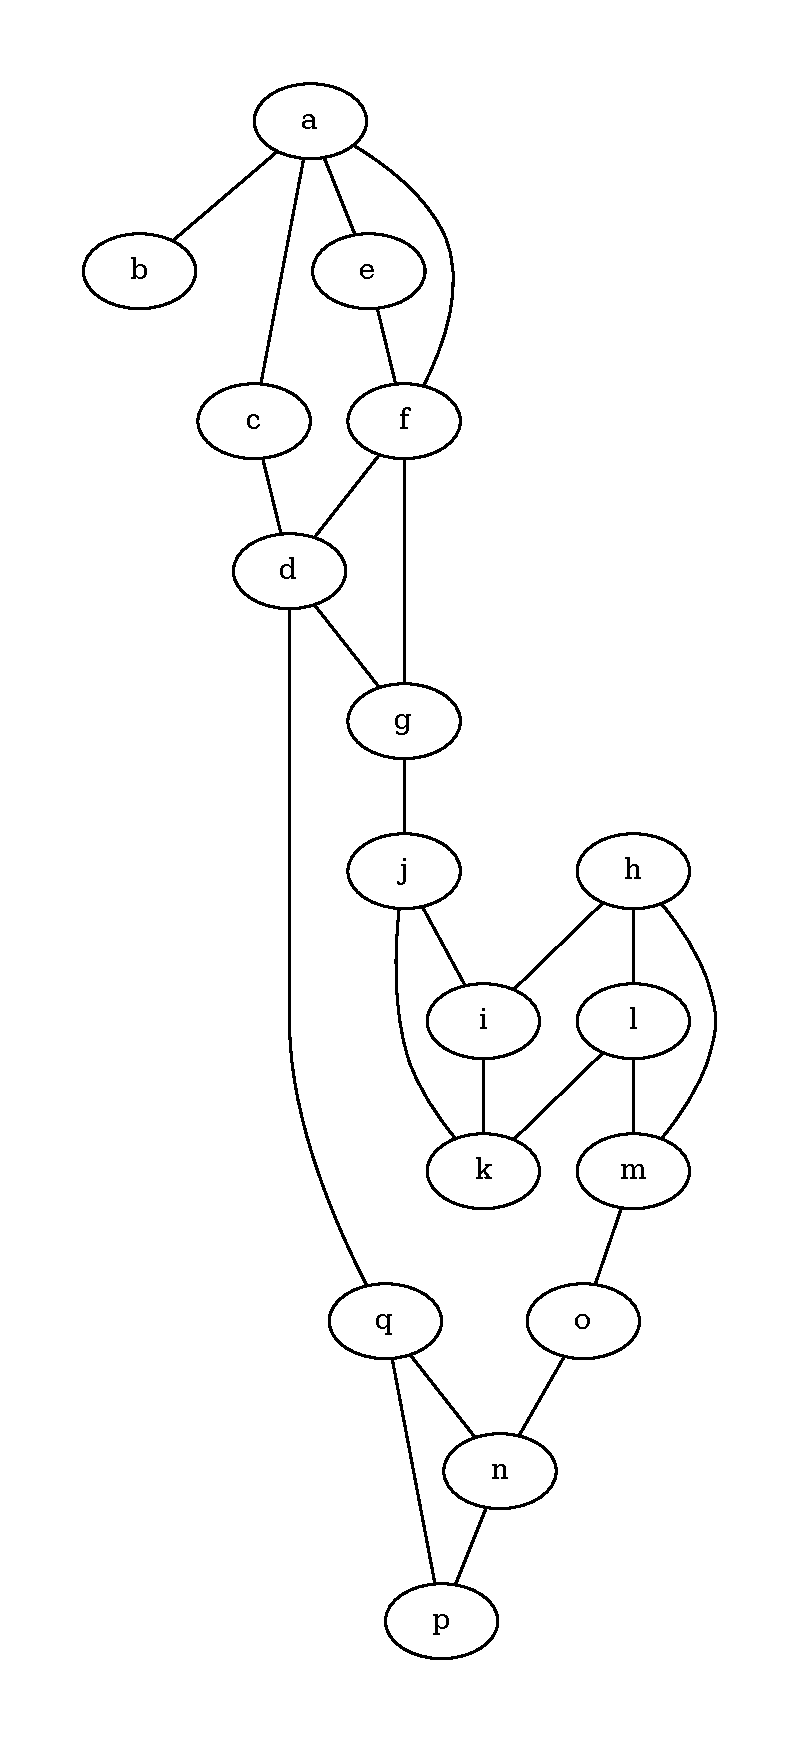
\includegraphics[width=0.8\textwidth]{imagens/render/GRAFO_3.png}
\end{center}

\subsubsection*{Atividade A.1: Criação a partir da Lista de Adjacências}
A estrutura do grafo é definida pela seguinte lista de adjacências:
\begin{itemize}[leftmargin=*]
    \item[\textbf{a:}] ['b', 'c', 'e', 'f'] \item[\textbf{b:}] ['a'] \item[\textbf{c:}] ['a', 'd'] \item[\textbf{d:}] ['c', 'f', 'g', 'q']
    \item[\textbf{e:}] ['a', 'f'] \item[\textbf{f:}] ['a', 'd', 'e', 'g'] \item[\textbf{g:}] ['d', 'f', 'j']
    \item[\textbf{h:}] ['i', 'l', 'm'] \item[\textbf{i:}] ['h', 'j', 'k'] \item[\textbf{j:}] ['g', 'i', 'k']
    \item[\textbf{k:}] ['i', 'j', 'l'] \item[\textbf{l:}] ['h', 'k', 'm'] \item[\textbf{m:}] ['h', 'l', 'o']
    \item[\textbf{n:}] ['o', 'p', 'q'] \item[\textbf{o:}] ['m', 'n'] \item[\textbf{p:}] ['n', 'q'] \item[\textbf{q:}] ['d', 'n', 'p']
\end{itemize}

\subsubsection*{Atividade A.2: Criação a partir da Matriz de Adjacências}
A estrutura do grafo é definida pela seguinte matriz de adjacências:
\begin{center}
\tiny
\begin{tabular*}{\textwidth}{c|@{\extracolsep{\fill}}ccccccccccccccccc}
\rowcolor[gray]{0.9}
 & \textbf{a} & \textbf{b} & \textbf{c} & \textbf{e} & \textbf{f} & \textbf{d} & \textbf{g} & \textbf{q} & \textbf{j} & \textbf{h} & \textbf{i} & \textbf{l} & \textbf{m} & \textbf{k} & \textbf{o} & \textbf{n} & \textbf{p} \\
\hline
\textbf{a} & 0 & 1 & 1 & 1 & 1 & 0 & 0 & 0 & 0 & 0 & 0 & 0 & 0 & 0 & 0 & 0 & 0 \\
\textbf{b} & 1 & 0 & 0 & 0 & 0 & 0 & 0 & 0 & 0 & 0 & 0 & 0 & 0 & 0 & 0 & 0 & 0 \\
\textbf{c} & 1 & 0 & 0 & 0 & 0 & 1 & 0 & 0 & 0 & 0 & 0 & 0 & 0 & 0 & 0 & 0 & 0 \\
\textbf{e} & 1 & 0 & 0 & 0 & 1 & 0 & 0 & 0 & 0 & 0 & 0 & 0 & 0 & 0 & 0 & 0 & 0 \\
\textbf{f} & 1 & 0 & 0 & 1 & 0 & 1 & 1 & 0 & 0 & 0 & 0 & 0 & 0 & 0 & 0 & 0 & 0 \\
\textbf{d} & 0 & 0 & 1 & 0 & 1 & 0 & 1 & 1 & 0 & 0 & 0 & 0 & 0 & 0 & 0 & 0 & 0 \\
\textbf{g} & 0 & 0 & 0 & 0 & 1 & 1 & 0 & 0 & 1 & 0 & 0 & 0 & 0 & 0 & 0 & 0 & 0 \\
\textbf{q} & 0 & 0 & 0 & 0 & 0 & 1 & 0 & 0 & 0 & 0 & 0 & 0 & 0 & 0 & 0 & 1 & 1 \\
\textbf{j} & 0 & 0 & 0 & 0 & 0 & 0 & 1 & 0 & 0 & 0 & 1 & 0 & 0 & 1 & 0 & 0 & 0 \\
\textbf{h} & 0 & 0 & 0 & 0 & 0 & 0 & 0 & 0 & 0 & 0 & 1 & 1 & 1 & 0 & 0 & 0 & 0 \\
\textbf{i} & 0 & 0 & 0 & 0 & 0 & 0 & 0 & 0 & 1 & 1 & 0 & 0 & 0 & 1 & 0 & 0 & 0 \\
\textbf{l} & 0 & 0 & 0 & 0 & 0 & 0 & 0 & 0 & 0 & 1 & 0 & 0 & 1 & 1 & 0 & 0 & 0 \\
\textbf{m} & 0 & 0 & 0 & 0 & 0 & 0 & 0 & 0 & 0 & 1 & 0 & 1 & 0 & 0 & 1 & 0 & 0 \\
\textbf{k} & 0 & 0 & 0 & 0 & 0 & 0 & 0 & 0 & 1 & 0 & 1 & 1 & 0 & 0 & 0 & 0 & 0 \\
\textbf{o} & 0 & 0 & 0 & 0 & 0 & 0 & 0 & 0 & 0 & 0 & 0 & 0 & 1 & 0 & 0 & 1 & 0 \\
\textbf{n} & 0 & 0 & 0 & 0 & 0 & 0 & 0 & 1 & 0 & 0 & 0 & 0 & 0 & 0 & 1 & 0 & 1 \\
\textbf{p} & 0 & 0 & 0 & 0 & 0 & 0 & 0 & 1 & 0 & 0 & 0 & 0 & 0 & 0 & 0 & 1 & 0 \\
\end{tabular*}
\end{center}

\subsubsection*{Atividade A.3: Criação a partir da Matriz de Incidência}
A matriz de incidência para o grafo (gerada a partir dos dados) mapeia vértices (linhas) a arestas (colunas). O grafo possui 24 arestas:
\begin{multicols}{4}
\begin{itemize}[nosep, leftmargin=*]
    \item[$e_1$:] (a,b) \item[$e_2$:] (a,c) \item[$e_3$:] (a,e) \item[$e_4$:] (a,f) \item[$e_5$:] (c,d) \item[$e_6$:] (d,f)
    \item[$e_7$:] (d,g) \item[$e_8$:] (d,q) \item[$e_9$:] (e,f) \item[$e_{10}$:] (f,g) \item[$e_{11}$:] (g,j) \item[$e_{12}$:] (h,i)
    \item[$e_{13}$:] (h,l) \item[$e_{14}$:] (h,m) \item[$e_{15}$:] (i,j) \item[$e_{16}$:] (i,k) \item[$e_{17}$:] (j,k) \item[$e_{18}$:] (k,l)
    \item[$e_{19}$:] (l,m) \item[$e_{20}$:] (m,o) \item[$e_{21}$:] (n,o) \item[$e_{22}$:] (n,p) \item[$e_{23}$:] (n,q) \item[$e_{24}$:] (p,q)
\end{itemize}
\end{multicols}
\begin{center}
\tiny
% Devido à extrema largura (24 arestas), esta tabela pode não renderizar perfeitamente.
\begin{tabular*}{\textwidth}{c|@{\extracolsep{\fill}}cccccccccccccccccccccccc}
\rowcolor[gray]{0.9}
 & \textbf{$e_1$} & \textbf{$e_2$} & \textbf{$e_3$} & \textbf{$e_4$} & \textbf{$e_5$} & \textbf{$e_6$} & \textbf{$e_7$} & \textbf{$e_8$} & \textbf{$e_9$} & \textbf{$e_{10}$} & \textbf{$e_{11}$} & \textbf{$e_{12}$} & \textbf{$e_{13}$} & \textbf{$e_{14}$} & \textbf{$e_{15}$} & \textbf{$e_{16}$} & \textbf{$e_{17}$} & \textbf{$e_{18}$} & \textbf{$e_{19}$} & \textbf{$e_{20}$} & \textbf{$e_{21}$} & \textbf{$e_{22}$} & \textbf{$e_{23}$} & \textbf{$e_{24}$} \\
\hline
\textbf{a} & 1&1&1&1&0&0&0&0&0&0&0&0&0&0&0&0&0&0&0&0&0&0&0&0 \\
\textbf{b} & 1&0&0&0&0&0&0&0&0&0&0&0&0&0&0&0&0&0&0&0&0&0&0&0 \\
\textbf{c} & 0&1&0&0&1&0&0&0&0&0&0&0&0&0&0&0&0&0&0&0&0&0&0&0 \\
\textbf{d} & 0&0&0&0&1&1&1&1&0&0&0&0&0&0&0&0&0&0&0&0&0&0&0&0 \\
\textbf{e} & 0&0&1&0&0&0&0&0&1&0&0&0&0&0&0&0&0&0&0&0&0&0&0&0 \\
\textbf{f} & 0&0&0&1&0&1&0&0&1&1&0&0&0&0&0&0&0&0&0&0&0&0&0&0 \\
\textbf{g} & 0&0&0&0&0&0&1&0&0&1&1&0&0&0&0&0&0&0&0&0&0&0&0&0 \\
\textbf{h} & 0&0&0&0&0&0&0&0&0&0&0&1&1&1&0&0&0&0&0&0&0&0&0&0 \\
\textbf{i} & 0&0&0&0&0&0&0&0&0&0&0&1&0&0&1&1&0&0&0&0&0&0&0&0 \\
\textbf{j} & 0&0&0&0&0&0&0&0&0&0&1&0&0&0&1&0&1&0&0&0&0&0&0&0 \\
\textbf{k} & 0&0&0&0&0&0&0&0&0&0&0&0&0&0&0&1&1&1&0&0&0&0&0&0 \\
\textbf{l} & 0&0&0&0&0&0&0&0&0&0&0&0&1&0&0&0&0&1&1&0&0&0&0&0 \\
\textbf{m} & 0&0&0&0&0&0&0&0&0&0&0&0&0&1&0&0&0&0&1&1&0&0&0&0 \\
\textbf{n} & 0&0&0&0&0&0&0&0&0&0&0&0&0&0&0&0&0&0&0&0&1&1&1&0 \\
\textbf{o} & 0&0&0&0&0&0&0&0&0&0&0&0&0&0&0&0&0&0&0&1&1&0&0&0 \\
\textbf{p} & 0&0&0&0&0&0&0&0&0&0&0&0&0&0&0&0&0&0&0&0&0&1&0&1 \\
\textbf{q} & 0&0&0&0&0&0&0&1&0&0&0&0&0&0&0&0&0&0&0&0&0&0&1&1 \\
\end{tabular*}
\end{center}

\subsubsection*{Atividade A.4: Conversão de Representações}
\paragraph*{Matriz de Adjacências $\rightarrow$ Lista de Adjacências:}
\begin{itemize}[leftmargin=*]
    \item[\textbf{a:}] ['b', 'c', 'e', 'f'] \item[\textbf{b:}] ['a'] \item[\textbf{c:}] ['a', 'd'] \item[\textbf{d:}] ['c', 'f', 'g', 'q']
    \item[\textbf{e:}] ['a', 'f'] \item[\textbf{f:}] ['a', 'd', 'e', 'g'] \item[\textbf{g:}] ['d', 'f', 'j']
    \item[\textbf{h:}] ['i', 'l', 'm'] \item[\textbf{i:}] ['h', 'j', 'k'] \item[\textbf{j:}] ['g', 'i', 'k']
    \item[\textbf{k:}] ['i', 'j', 'l'] \item[\textbf{l:}] ['h', 'k', 'm'] \item[\textbf{m:}] ['h', 'l', 'o']
    \item[\textbf{n:}] ['o', 'p', 'q'] \item[\textbf{o:}] ['m', 'n'] \item[\textbf{p:}] ['n', 'q'] \item[\textbf{q:}] ['d', 'n', 'p']
\end{itemize}
\paragraph*{Lista de Adjacências $\rightarrow$ Matriz de Adjacências:}
\begin{center}
\tiny
\begin{tabular*}{\textwidth}{c|@{\extracolsep{\fill}}ccccccccccccccccc}
\rowcolor[gray]{0.9}
 & \textbf{a} & \textbf{b} & \textbf{c} & \textbf{e} & \textbf{f} & \textbf{d} & \textbf{g} & \textbf{q} & \textbf{j} & \textbf{h} & \textbf{i} & \textbf{l} & \textbf{m} & \textbf{k} & \textbf{o} & \textbf{n} & \textbf{p} \\ \hline
\textbf{a} & 0&1&1&1&1&0&0&0&0&0&0&0&0&0&0&0&0 \\ \textbf{b} & 1&0&0&0&0&0&0&0&0&0&0&0&0&0&0&0&0 \\
\textbf{c} & 1&0&0&0&0&1&0&0&0&0&0&0&0&0&0&0&0 \\ \textbf{e} & 1&0&0&0&1&0&0&0&0&0&0&0&0&0&0&0&0 \\
\textbf{f} & 1&0&0&1&0&1&1&0&0&0&0&0&0&0&0&0&0 \\ \textbf{d} & 0&0&1&0&1&0&1&1&0&0&0&0&0&0&0&0&0 \\
\textbf{g} & 0&0&0&0&1&1&0&0&1&0&0&0&0&0&0&0&0 \\ \textbf{q} & 0&0&0&0&0&1&0&0&0&0&0&0&0&0&0&1&1 \\
\textbf{j} & 0&0&0&0&0&0&1&0&0&0&1&0&0&1&0&0&0 \\ \textbf{h} & 0&0&0&0&0&0&0&0&0&0&1&1&1&0&0&0&0 \\
\textbf{i} & 0&0&0&0&0&0&0&0&1&1&0&0&0&1&0&0&0 \\ \textbf{l} & 0&0&0&0&0&0&0&0&0&1&0&0&1&1&0&0&0 \\
\textbf{m} & 0&0&0&0&0&0&0&0&0&1&0&1&0&0&1&0&0 \\ \textbf{k} & 0&0&0&0&0&0&0&0&1&0&1&1&0&0&0&0&0 \\
\textbf{o} & 0&0&0&0&0&0&0&0&0&0&0&0&1&0&0&1&0 \\ \textbf{n} & 0&0&0&0&0&0&0&1&0&0&0&0&0&0&1&0&1 \\
\textbf{p} & 0&0&0&0&0&0&0&1&0&0&0&0&0&0&0&1&0 \\
\end{tabular*}
\end{center}

\subsubsection*{Atividade A.5: Cálculo do Grau dos Vértices}
\begin{multicols}{3}
\begin{itemize}[nosep]
    \item $d(a) = 4$ \item $d(b) = 1$ \item $d(c) = 2$
    \item $d(d) = 4$ \item $d(e) = 2$ \item $d(f) = 4$
    \item $d(g) = 3$ \item $d(h) = 3$ \item $d(i) = 3$
    \item $d(j) = 3$ \item $d(k) = 3$ \item $d(l) = 3$
    \item $d(m) = 3$ \item $d(n) = 3$ \item $d(o) = 2$
    \item $d(p) = 2$ \item $d(q) = 3$
\end{itemize}
\end{multicols}

\subsubsection*{Atividade A.6: Adjacência entre Vértices}
\begin{itemize}[align=left, leftmargin=40pt, labelsep=1em]
    \item[Adjacentes de a:] ['b', 'c', 'e', 'f']
    \item[Adjacentes de b:] ['a']
    \item[Adjacentes de c:] ['a', 'd']
    \item[Adjacentes de d:] ['c', 'f', 'g', 'q']
    \item[Adjacentes de e:] ['a', 'f']
    \item[Adjacentes de f:] ['a', 'd', 'e', 'g']
    \item[Adjacentes de g:] ['d', 'f', 'j']
    \item[Adjacentes de h:] ['i', 'l', 'm']
    \item[Adjacentes de i:] ['h', 'j', 'k']
    \item[Adjacentes de j:] ['g', 'i', 'k']
    \item[Adjacentes de k:] ['i', 'j', 'l']
    \item[Adjacentes de l:] ['h', 'k', 'm']
    \item[Adjacentes de m:] ['h', 'l', 'o']
    \item[Adjacentes de n:] ['o', 'p', 'q']
    \item[Adjacentes de o:] ['m', 'n']
    \item[Adjacentes de p:] ['n', 'q']
    \item[Adjacentes de q:] ['d', 'n', 'p']
\end{itemize}

\subsubsection*{Atividade A.7: Número Total de Vértices}
O grafo possui \textbf{17} vértices.

\subsubsection*{Atividade A.8: Número Total de Arestas}
O grafo possui \textbf{24} arestas.

\subsubsection*{Atividade A.9: Inclusão de Vértice}
\textit{Esta operação não foi demonstrada no arquivo de análise.}

\subsubsection*{Atividade A.10: Exclusão de Vértice}
\textit{Esta operação não foi demonstrada no arquivo de análise.}

\subsubsection*{Atividade A.11: Verificação de Conectividade}
O grafo é \textbf{conexo}.

\subsubsection*{Atividade A.12: Verificação de Bipartição}
O grafo \textbf{não} é bipartido.

\subsubsection*{Atividade A.13: Busca em Largura (BFS)}
\begin{center}
    \includegraphics[width=0.7\textwidth]{imagens/render/bfs/GRAFO_3_BFS.png}
\end{center}

\subsubsection*{Atividade A.14: Busca em Profundidade (DFS)}
\begin{center}
    \includegraphics[width=0.6\textwidth]{imagens/render/dfs/GRAFO_3_DFS.png}
\end{center}

\subsubsection*{Atividade A.15: Determinação de Articulações e Blocos}
\begin{itemize}[nosep, leftmargin=*]
    \item \textbf{Pontos de Articulação (Vértices de Corte):} ['a']
    \item \textbf{Pontes:} [('a', 'b')]
\end{itemize}

\\ 

% =====================================================================
% =================== SEÇÃO PARA DIGRAFOS =============================
% =====================================================================
\section{Análise dos Dígrafos}

% ----------------- DIGRAFO_0.txt -----------------
\subsection{Resultados para o arquivo: DIGRAFO\_0.txt}

\begin{center}
    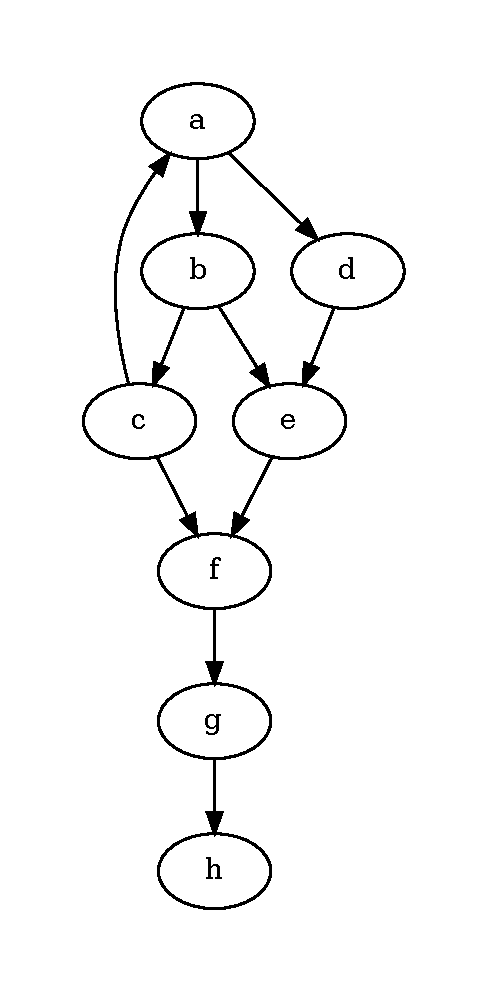
\includegraphics[width=0.4\textwidth]{imagens/render/DIGRAFO_0.png}
\end{center}

\subsubsection*{Atividade B.16: Representação por Matriz de Adjacências}
\begin{center}
\scriptsize
\begin{tabular*}{\textwidth}{c|@{\extracolsep{\fill}}cccccccc}
\rowcolor[gray]{0.9}
  & \textbf{a} & \textbf{b} & \textbf{d} & \textbf{c} & \textbf{e} & \textbf{f} & \textbf{g} & \textbf{h} \\
\hline
\textbf{a} & 0 & 1 & 1 & 0 & 0 & 0 & 0 & 0 \\
\textbf{b} & 0 & 0 & 0 & 1 & 1 & 0 & 0 & 0 \\
\textbf{d} & 0 & 0 & 0 & 0 & 1 & 0 & 0 & 0 \\
\textbf{c} & 1 & 0 & 0 & 0 & 0 & 1 & 0 & 0 \\
\textbf{e} & 0 & 0 & 0 & 0 & 0 & 1 & 0 & 0 \\
\textbf{f} & 0 & 0 & 0 & 0 & 0 & 0 & 1 & 0 \\
\textbf{g} & 0 & 0 & 0 & 0 & 0 & 0 & 0 & 1 \\
\textbf{h} & 0 & 0 & 0 & 0 & 0 & 0 & 0 & 0 \\
\end{tabular*}
\end{center}

\subsubsection*{Atividade B.17: Representação por Matriz de Incidência}
A matriz de incidência para dígrafos mapeia vértices (linhas) a arestas (colunas), usando a convenção: \textbf{+1} para a origem da aresta e \textbf{-1} para o destino. O dígrafo possui 10 arestas:
\begin{multicols}{2}
\begin{itemize}[nosep, leftmargin=*]
    \item[$e_1$:] (a,b)
    \item[$e_2$:] (a,d)
    \item[$e_3$:] (b,c)
    \item[$e_4$:] (b,e)
    \item[$e_5$:] (d,e)
    \item[$e_6$:] (c,a)
    \item[$e_7$:] (c,f)
    \item[$e_8$:] (e,f)
    \item[$e_9$:] (f,g)
    \item[$e_{10}$:] (g,h)
\end{itemize}
\end{multicols}
\begin{center}
\scriptsize
\begin{tabular*}{\textwidth}{c|@{\extracolsep{\fill}}cccccccccc}
\rowcolor[gray]{0.9}
 & \textbf{$e_1$} & \textbf{$e_2$} & \textbf{$e_3$} & \textbf{$e_4$} & \textbf{$e_5$} & \textbf{$e_6$} & \textbf{$e_7$} & \textbf{$e_8$} & \textbf{$e_9$} & \textbf{$e_{10}$} \\
\hline
\textbf{a} &  1 &  1 &  0 &  0 &  0 & -1 &  0 &  0 &  0 &  0 \\
\textbf{b} & -1 &  0 &  1 &  1 &  0 &  0 &  0 &  0 &  0 &  0 \\
\textbf{c} &  0 &  0 & -1 &  0 &  0 &  1 &  1 &  0 &  0 &  0 \\
\textbf{d} &  0 & -1 &  0 &  0 &  1 &  0 &  0 &  0 &  0 &  0 \\
\textbf{e} &  0 &  0 &  0 & -1 & -1 &  0 &  0 &  1 &  0 &  0 \\
\textbf{f} &  0 &  0 &  0 &  0 &  0 &  0 & -1 & -1 &  1 &  0 \\
\textbf{g} &  0 &  0 &  0 &  0 &  0 &  0 &  0 &  0 & -1 &  1 \\
\textbf{h} &  0 &  0 &  0 &  0 &  0 &  0 &  0 &  0 &  0 & -1 \\
\end{tabular*}
\end{center}

\subsubsection*{Graus de Entrada e Saída}
\begin{multicols}{3}
\begin{itemize}[nosep]
    \item $d^{+}(a)=2, d^{-}(a)=1$
    \item $d^{+}(b)=2, d^{-}(b)=1$
    \item $d^{+}(c)=2, d^{-}(c)=1$
    \item $d^{+}(d)=1, d^{-}(d)=1$
    \item $d^{+}(e)=1, d^{-}(e)=2$
    \item $d^{+}(f)=1, d^{-}(f)=2$
    \item $d^{+}(g)=1, d^{-}(g)=1$
    \item $d^{+}(h)=0, d^{-}(h)=1$
\end{itemize}
\end{multicols}

\subsubsection*{Sucessores e Antecessores}
\begin{itemize}[leftmargin=*]
    \item[\textbf{a:}] \textbf{Sucessores:} ['b', 'd'], \textbf{Antecessores:} ['c']
    \item[\textbf{b:}] \textbf{Sucessores:} ['c', 'e'], \textbf{Antecessores:} ['a']
    \item[\textbf{c:}] \textbf{Sucessores:} ['a', 'f'], \textbf{Antecessores:} ['b']
    \item[\textbf{d:}] \textbf{Sucessores:} ['e'], \textbf{Antecessores:} ['a']
    \item[\textbf{e:}] \textbf{Sucessores:} ['f'], \textbf{Antecessores:} ['b', 'd']
    \item[\textbf{f:}] \textbf{Sucessores:} ['g'], \textbf{Antecessores:} ['c', 'e']
    \item[\textbf{g:}] \textbf{Sucessores:} ['h'], \textbf{Antecessores:} ['f']
    \item[\textbf{h:}] \textbf{Sucessores:} [], \textbf{Antecessores:} ['g']
\end{itemize}

\subsubsection*{Atividade B.18: Determinação do Grafo Subjacente}
O grafo subjacente é um grafo não-direcionado obtido ao remover a direcionalidade de todas as arestas do dígrafo. Sua representação por lista de adjacência é:
\begin{itemize}[leftmargin=*]
    \item[\textbf{a:}] ['b', 'c', 'd']
    \item[\textbf{b:}] ['a', 'c', 'e']
    \item[\textbf{c:}] ['a', 'b', 'f']
    \item[\textbf{d:}] ['a', 'e']
    \item[\textbf{e:}] ['b', 'd', 'f']
    \item[\textbf{f:}] ['c', 'e', 'g']
    \item[\textbf{g:}] ['f', 'h']
    \item[\textbf{h:}] ['g']
\end{itemize}

\begin{center}
    \includegraphics[width=0.4\textwidth]{imagens/render/subjacente/SUBJACENTE_DIGRAFO_0.png}
\end{center}


\subsubsection*{Atividade B.19: Busca em Largura (BFS)}
\begin{center}
    \includegraphics[width=0.4\textwidth]{imagens/render/bfs/DIGRAFO_0_BFS.png}
\end{center}

\subsubsection*{Atividade B.20: Busca em Profundidade (DFS)}
\begin{center}
    \includegraphics[width=0.3\textwidth]{imagens/render/dfs/DIGRAFO_0_DFS.png}
\end{center}
\\
% ----------------- DIGRAFO1.txt -----------------
\subsection{Resultados para o arquivo: DIGRAFO\_1.txt}

\begin{center}
    \includegraphics[width=0.8\textwidth]{imagens/render/DIGRAFO_1.png}
\end{center}

\subsubsection*{Atividade B.16: Representação por Matriz de Adjacências}
\begin{center}
\tiny
\begin{tabular*}{\textwidth}{c|@{\extracolsep{\fill}}ccccccccccccc}
\rowcolor[gray]{0.9}
 & \textbf{1} & \textbf{2} & \textbf{3} & \textbf{4} & \textbf{5} & \textbf{6} & \textbf{8} & \textbf{7} & \textbf{9} & \textbf{10} & \textbf{11} & \textbf{12} & \textbf{13} \\
\hline
\textbf{1} & 0 & 1 & 0 & 0 & 0 & 0 & 0 & 0 & 0 & 0 & 0 & 0 & 0 \\
\textbf{2} & 0 & 0 & 1 & 0 & 0 & 0 & 0 & 0 & 0 & 0 & 0 & 0 & 0 \\
\textbf{3} & 1 & 0 & 0 & 1 & 0 & 0 & 0 & 0 & 0 & 0 & 0 & 0 & 0 \\
\textbf{4} & 0 & 0 & 0 & 0 & 1 & 0 & 0 & 0 & 0 & 0 & 0 & 0 & 0 \\
\textbf{5} & 0 & 0 & 0 & 0 & 0 & 1 & 1 & 0 & 0 & 0 & 0 & 0 & 0 \\
\textbf{6} & 0 & 0 & 0 & 0 & 0 & 0 & 0 & 1 & 0 & 0 & 0 & 0 & 0 \\
\textbf{8} & 0 & 0 & 0 & 1 & 0 & 0 & 0 & 0 & 0 & 1 & 0 & 0 & 0 \\
\textbf{7} & 0 & 0 & 0 & 0 & 0 & 1 & 0 & 0 & 1 & 0 & 0 & 0 & 0 \\
\textbf{9} & 0 & 0 & 0 & 0 & 0 & 0 & 1 & 0 & 0 & 0 & 0 & 0 & 0 \\
\textbf{10} & 0 & 0 & 0 & 0 & 0 & 0 & 0 & 0 & 0 & 0 & 0 & 0 & 0 \\
\textbf{11} & 0 & 0 & 0 & 0 & 0 & 0 & 0 & 0 & 0 & 0 & 0 & 1 & 0 \\
\textbf{12} & 0 & 0 & 0 & 0 & 0 & 0 & 0 & 0 & 0 & 0 & 0 & 0 & 1 \\
\textbf{13} & 0 & 0 & 0 & 0 & 0 & 0 & 0 & 0 & 0 & 0 & 0 & 1 & 0 \\
\end{tabular*}
\end{center}

\subsubsection*{Atividade B.17: Representação por Matriz de Incidência}
A matriz de incidência para dígrafos mapeia vértices (linhas) a arestas (colunas), usando a convenção: \textbf{+1} para a origem da aresta e \textbf{-1} para o destino. O dígrafo possui 16 arestas:
\begin{multicols}{3}
\begin{itemize}[nosep, leftmargin=*]
    \item[$e_1$:] (1,2) \item[$e_2$:] (2,3) \item[$e_3$:] (3,1) \item[$e_4$:] (3,4) \item[$e_5$:] (4,5) \item[$e_6$:] (5,6)
    \item[$e_7$:] (5,8) \item[$e_8$:] (6,7) \item[$e_9$:] (7,6) \item[$e_{10}$:] (7,9) \item[$e_{11}$:] (8,10) \item[$e_{12}$:] (8,4)
    \item[$e_{13}$:] (9,8) \item[$e_{14}$:] (11,12) \item[$e_{15}$:] (12,13) \item[$e_{16}$:] (13,12)
\end{itemize}
\end{multicols}
\begin{center}
\tiny
\begin{tabular*}{\textwidth}{c|@{\extracolsep{\fill}}cccccccccccccccc}
\rowcolor[gray]{0.9}
 & \textbf{$e_1$} & \textbf{$e_2$} & \textbf{$e_3$} & \textbf{$e_4$} & \textbf{$e_5$} & \textbf{$e_6$} & \textbf{$e_7$} & \textbf{$e_8$} & \textbf{$e_9$} & \textbf{$e_{10}$} & \textbf{$e_{11}$} & \textbf{$e_{12}$} & \textbf{$e_{13}$} & \textbf{$e_{14}$} & \textbf{$e_{15}$} & \textbf{$e_{16}$} \\
\hline
\textbf{1}  &  1 &  0 & -1 &  0 &  0 &  0 &  0 &  0 &  0 &  0 &  0 &  0 &  0 &  0 &  0 &  0 \\
\textbf{2}  & -1 &  1 &  0 &  0 &  0 &  0 &  0 &  0 &  0 &  0 &  0 &  0 &  0 &  0 &  0 &  0 \\
\textbf{3}  &  0 & -1 &  1 &  1 &  0 &  0 &  0 &  0 &  0 &  0 &  0 &  0 &  0 &  0 &  0 &  0 \\
\textbf{4}  &  0 &  0 &  0 & -1 &  1 &  0 &  0 &  0 &  0 &  0 &  0 & -1 &  0 &  0 &  0 &  0 \\
\textbf{5}  &  0 &  0 &  0 &  0 & -1 &  1 &  1 &  0 &  0 &  0 &  0 &  0 &  0 &  0 &  0 &  0 \\
\textbf{6}  &  0 &  0 &  0 &  0 &  0 & -1 &  0 &  1 & -1 &  0 &  0 &  0 &  0 &  0 &  0 &  0 \\
\textbf{7}  &  0 &  0 &  0 &  0 &  0 &  0 &  0 & -1 &  1 &  1 &  0 &  0 &  0 &  0 &  0 &  0 \\
\textbf{8}  &  0 &  0 &  0 &  0 &  0 &  0 & -1 &  0 &  0 &  0 &  1 &  1 & -1 &  0 &  0 &  0 \\
\textbf{9}  &  0 &  0 &  0 &  0 &  0 &  0 &  0 &  0 &  0 & -1 &  0 &  0 &  1 &  0 &  0 &  0 \\
\textbf{10} &  0 &  0 &  0 &  0 &  0 &  0 &  0 &  0 &  0 &  0 & -1 &  0 &  0 &  0 &  0 &  0 \\
\textbf{11} &  0 &  0 &  0 &  0 &  0 &  0 &  0 &  0 &  0 &  0 &  0 &  0 &  0 &  1 &  0 &  0 \\
\textbf{12} &  0 &  0 &  0 &  0 &  0 &  0 &  0 &  0 &  0 &  0 &  0 &  0 &  0 & -1 &  1 & -1 \\
\textbf{13} &  0 &  0 &  0 &  0 &  0 &  0 &  0 &  0 &  0 &  0 &  0 &  0 &  0 &  0 & -1 &  1 \\
\end{tabular*}
\end{center}

% --- SEÇÃO ADICIONADA ---
\subsubsection*{Graus de Entrada e Saída}
\begin{multicols}{3}
\begin{itemize}[nosep]
    \item $d^{+}(1)=1, d^{-}(1)=1$
    \item $d^{+}(2)=1, d^{-}(2)=1$
    \item $d^{+}(3)=2, d^{-}(3)=1$
    \item $d^{+}(4)=1, d^{-}(4)=2$
    \item $d^{+}(5)=2, d^{-}(5)=1$
    \item $d^{+}(6)=1, d^{-}(6)=2$
    \item $d^{+}(7)=2, d^{-}(7)=1$
    \item $d^{+}(8)=2, d^{-}(8)=2$
    \item $d^{+}(9)=1, d^{-}(9)=1$
    \item $d^{+}(10)=0, d^{-}(10)=1$
    \item $d^{+}(11)=1, d^{-}(11)=0$
    \item $d^{+}(12)=1, d^{-}(12)=2$
    \item $d^{+}(13)=1, d^{-}(13)=1$
\end{itemize}
\end{multicols}

% --- SEÇÃO ADICIONADA ---
\subsubsection*{Sucessores e Antecessores}
\begin{itemize}[leftmargin=*]
    \item[\textbf{1:}] \textbf{Sucessores:} ['2'], \textbf{Antecessores:} ['3']
    \item[\textbf{2:}] \textbf{Sucessores:} ['3'], \textbf{Antecessores:} ['1']
    \item[\textbf{3:}] \textbf{Sucessores:} ['1', '4'], \textbf{Antecessores:} ['2']
    \item[\textbf{4:}] \textbf{Sucessores:} ['5'], \textbf{Antecessores:} ['3', '8']
    \item[\textbf{5:}] \textbf{Sucessores:} ['6', '8'], \textbf{Antecessores:} ['4']
    \item[\textbf{6:}] \textbf{Sucessores:} ['7'], \textbf{Antecessores:} ['5', '7']
    \item[\textbf{7:}] \textbf{Sucessores:} ['6', '9'], \textbf{Antecessores:} ['6']
    \item[\textbf{8:}] \textbf{Sucessores:} ['10', '4'], \textbf{Antecessores:} ['5', '9']
    \item[\textbf{9:}] \textbf{Sucessores:} ['8'], \textbf{Antecessores:} ['7']
    \item[\textbf{10:}] \textbf{Sucessores:} [], \textbf{Antecessores:} ['8']
    \item[\textbf{11:}] \textbf{Sucessores:} ['12'], \textbf{Antecessores:} []
    \item[\textbf{12:}] \textbf{Sucessores:} ['13'], \textbf{Antecessores:} ['11', '13']
    \item[\textbf{13:}] \textbf{Sucessores:} ['12'], \textbf{Antecessores:} ['12']
\end{itemize}

\subsubsection*{Atividade B.18: Determinação do Grafo Subjacente}
O grafo subjacente é um grafo não-direcionado obtido ao remover a direcionalidade de todas as arestas do dígrafo. Sua representação por lista de adjacência é:
\begin{itemize}[leftmargin=*]
    \item[\textbf{1:}] ['2', '3']
    \item[\textbf{2:}] ['1', '3']
    \item[\textbf{3:}] ['1', '2', '4']
    \item[\textbf{4:}] ['3', '5', '8']
    \item[\textbf{5:}] ['4', '6', '8']
    \item[\textbf{6:}] ['5', '7']
    \item[\textbf{7:}] ['6', '9']
    \item[\textbf{8:}] ['4', '5', '9', '10']
    \item[\textbf{9:}] ['7', '8']
    \item[\textbf{10:}] ['8']
    \item[\textbf{11:}] ['12']
    \item[\textbf{12:}] ['11', '13']
    \item[\textbf{13:}] ['12']
\end{itemize}

\begin{center}
    \includegraphics[width=0.9\textwidth]{imagens/render/subjacente/SUBJACENTE_DIGRAFO_1.png}
\end{center}

\subsubsection*{Atividade B.19: Busca em Largura (BFS)}
\begin{center}
    \includegraphics[width=0.4\textwidth]{imagens/render/bfs/DIGRAFO_1_BFS.png}
\end{center}

\subsubsection*{Atividade B.20: Busca em Profundidade (DFS)}
\begin{center}
    \includegraphics[width=0.3\textwidth]{imagens/render/dfs/DIGRAFO_1_DFS.png}
\end{center}
\\

% ----------------- DIGRAFO2.txt -----------------
\subsection{Resultados para o arquivo: DIGRAFO\_2.txt}

\begin{center}
    \includegraphics[width=0.6\textwidth]{imagens/render/DIGRAFO_2.png}
\end{center}

\subsubsection*{Atividade B.16: Representação por Matriz de Adjacências}
\begin{center}
\scriptsize 
\begin{tabular*}{\textwidth}{c|@{\extracolsep{\fill}}ccccccccccccc}
\rowcolor[gray]{0.9}
 & \textbf{1} & \textbf{2} & \textbf{3} & \textbf{4} & \textbf{5} & \textbf{6} & \textbf{8} & \textbf{7} & \textbf{9} & \textbf{10} & \textbf{12} & \textbf{11} & \textbf{13} \\
\hline
\textbf{1} & 0 & 1 & 0 & 0 & 0 & 0 & 0 & 0 & 0 & 0 & 0 & 0 & 0 \\
\textbf{2} & 0 & 0 & 1 & 0 & 0 & 0 & 0 & 0 & 0 & 0 & 0 & 0 & 0 \\
\textbf{3} & 1 & 0 & 0 & 1 & 0 & 0 & 0 & 0 & 0 & 0 & 0 & 0 & 0 \\
\textbf{4} & 0 & 0 & 0 & 0 & 1 & 0 & 0 & 0 & 0 & 0 & 0 & 0 & 0 \\
\textbf{5} & 0 & 0 & 0 & 0 & 0 & 1 & 1 & 0 & 0 & 0 & 0 & 0 & 0 \\
\textbf{6} & 0 & 0 & 0 & 0 & 0 & 0 & 0 & 1 & 0 & 0 & 0 & 0 & 0 \\
\textbf{8} & 0 & 0 & 0 & 1 & 0 & 0 & 0 & 0 & 0 & 1 & 0 & 0 & 0 \\
\textbf{7} & 0 & 0 & 0 & 0 & 0 & 1 & 0 & 0 & 1 & 0 & 0 & 0 & 0 \\
\textbf{9} & 0 & 0 & 0 & 0 & 0 & 0 & 1 & 0 & 0 & 0 & 0 & 0 & 0 \\
\textbf{10} & 0 & 0 & 0 & 0 & 0 & 0 & 0 & 0 & 0 & 0 & 1 & 0 & 0 \\
\textbf{12} & 0 & 0 & 0 & 0 & 0 & 0 & 0 & 0 & 0 & 0 & 0 & 0 & 1 \\
\textbf{11} & 0 & 0 & 0 & 0 & 0 & 0 & 0 & 0 & 0 & 0 & 1 & 0 & 0 \\
\textbf{13} & 0 & 0 & 0 & 0 & 0 & 0 & 0 & 0 & 0 & 0 & 1 & 0 & 0 \\
\end{tabular*}
\end{center}

\subsubsection*{Atividade B.17: Representação por Matriz de Incidência}
A matriz de incidência para dígrafos mapeia vértices (linhas) a arestas (colunas), usando a convenção: \textbf{+1} para a origem da aresta e \textbf{-1} para o destino. O dígrafo possui 17 arestas:
\begin{multicols}{3}
\begin{itemize}[nosep, leftmargin=*]
    \item[$e_1$:] (1,2)
    \item[$e_2$:] (2,3)
    \item[$e_3$:] (3,1)
    \item[$e_4$:] (3,4)
    \item[$e_5$:] (4,5)
    \item[$e_6$:] (5,6)
    \item[$e_7$:] (5,8)
    \item[$e_8$:] (6,7)
    \item[$e_9$:] (7,6)
    \item[$e_{10}$:] (7,9)
    \item[$e_{11}$:] (8,10)
    \item[$e_{12}$:] (8,4)
    \item[$e_{13}$:] (9,8)
    \item[$e_{14}$:] (10,12)
    \item[$e_{15}$:] (11,12)
    \item[$e_{16}$:] (12,13)
    \item[$e_{17}$:] (13,12)
\end{itemize}
\end{multicols}
\begin{center}
\tiny
\begin{tabular*}{\textwidth}{c|@{\extracolsep{\fill}}ccccccccccccccccc}
\rowcolor[gray]{0.9}
 & \textbf{$e_1$} & \textbf{$e_2$} & \textbf{$e_3$} & \textbf{$e_4$} & \textbf{$e_5$} & \textbf{$e_6$} & \textbf{$e_7$} & \textbf{$e_8$} & \textbf{$e_9$} & \textbf{$e_{10}$} & \textbf{$e_{11}$} & \textbf{$e_{12}$} & \textbf{$e_{13}$} & \textbf{$e_{14}$} & \textbf{$e_{15}$} & \textbf{$e_{16}$} & \textbf{$e_{17}$} \\
\hline
\textbf{1}  &  1 &  0 & -1 &  0 &  0 &  0 &  0 &  0 &  0 &  0 &  0 &  0 &  0 &  0 &  0 &  0 &  0 \\
\textbf{2}  & -1 &  1 &  0 &  0 &  0 &  0 &  0 &  0 &  0 &  0 &  0 &  0 &  0 &  0 &  0 &  0 &  0 \\
\textbf{3}  &  0 & -1 &  1 &  1 &  0 &  0 &  0 &  0 &  0 &  0 &  0 &  0 &  0 &  0 &  0 &  0 &  0 \\
\textbf{4}  &  0 &  0 &  0 & -1 &  1 &  0 &  0 &  0 &  0 &  0 &  0 & -1 &  0 &  0 &  0 &  0 &  0 \\
\textbf{5}  &  0 &  0 &  0 &  0 & -1 &  1 &  1 &  0 &  0 &  0 &  0 &  0 &  0 &  0 &  0 &  0 &  0 \\
\textbf{6}  &  0 &  0 &  0 &  0 &  0 & -1 &  0 &  1 & -1 &  0 &  0 &  0 &  0 &  0 &  0 &  0 &  0 \\
\textbf{7}  &  0 &  0 &  0 &  0 &  0 &  0 &  0 & -1 &  1 &  1 &  0 &  0 &  0 &  0 &  0 &  0 &  0 \\
\textbf{8}  &  0 &  0 &  0 &  0 &  0 &  0 & -1 &  0 &  0 &  0 &  1 &  1 & -1 &  0 &  0 &  0 &  0 \\
\textbf{9}  &  0 &  0 &  0 &  0 &  0 &  0 &  0 &  0 &  0 & -1 &  0 &  0 &  1 &  0 &  0 &  0 &  0 \\
\textbf{10} &  0 &  0 &  0 &  0 &  0 &  0 &  0 &  0 &  0 &  0 & -1 &  0 &  0 &  1 &  0 &  0 &  0 \\
\textbf{11} &  0 &  0 &  0 &  0 &  0 &  0 &  0 &  0 &  0 &  0 &  0 &  0 &  0 &  0 &  1 &  0 &  0 \\
\textbf{12} &  0 &  0 &  0 &  0 &  0 &  0 &  0 &  0 &  0 &  0 &  0 &  0 &  0 & -1 & -1 &  1 & -1 \\
\textbf{13} &  0 &  0 &  0 &  0 &  0 &  0 &  0 &  0 &  0 &  0 &  0 &  0 &  0 &  0 &  0 & -1 &  1 \\
\end{tabular*}
\end{center}

% --- SEÇÃO ADICIONADA ---
\subsubsection*{Graus de Entrada e Saída}
\begin{multicols}{3}
\begin{itemize}[nosep]
    \item $d^{+}(1)=1, d^{-}(1)=1$
    \item $d^{+}(2)=1, d^{-}(2)=1$
    \item $d^{+}(3)=2, d^{-}(3)=1$
    \item $d^{+}(4)=1, d^{-}(4)=2$
    \item $d^{+}(5)=2, d^{-}(5)=1$
    \item $d^{+}(6)=1, d^{-}(6)=2$
    \item $d^{+}(7)=2, d^{-}(7)=1$
    \item $d^{+}(8)=2, d^{-}(8)=2$
    \item $d^{+}(9)=1, d^{-}(9)=1$
    \item $d^{+}(10)=1, d^{-}(10)=1$
    \item $d^{+}(11)=1, d^{-}(11)=0$
    \item $d^{+}(12)=1, d^{-}(12)=3$
    \item $d^{+}(13)=1, d^{-}(13)=1$
\end{itemize}
\end{multicols}

% --- SEÇÃO ADICIONADA ---
\subsubsection*{Sucessores e Antecessores}
\begin{itemize}[leftmargin=*]
    \item[\textbf{1:}] \textbf{Sucessores:} ['2'], \textbf{Antecessores:} ['3']
    \item[\textbf{2:}] \textbf{Sucessores:} ['3'], \textbf{Antecessores:} ['1']
    \item[\textbf{3:}] \textbf{Sucessores:} ['1', '4'], \textbf{Antecessores:} ['2']
    \item[\textbf{4:}] \textbf{Sucessores:} ['5'], \textbf{Antecessores:} ['3', '8']
    \item[\textbf{5:}] \textbf{Sucessores:} ['6', '8'], \textbf{Antecessores:} ['4']
    \item[\textbf{6:}] \textbf{Sucessores:} ['7'], \textbf{Antecessores:} ['5', '7']
    \item[\textbf{7:}] \textbf{Sucessores:} ['6', '9'], \textbf{Antecessores:} ['6']
    \item[\textbf{8:}] \textbf{Sucessores:} ['10', '4'], \textbf{Antecessores:} ['5', '9']
    \item[\textbf{9:}] \textbf{Sucessores:} ['8'], \textbf{Antecessores:} ['7']
    \item[\textbf{10:}] \textbf{Sucessores:} ['12'], \textbf{Antecessores:} ['8']
    \item[\textbf{11:}] \textbf{Sucessores:} ['12'], \textbf{Antecessores:} []
    \item[\textbf{12:}] \textbf{Sucessores:} ['13'], \textbf{Antecessores:} ['10', '11', '13']
    \item[\textbf{13:}] \textbf{Sucessores:} ['12'], \textbf{Antecessores:} ['12']
\end{itemize}

\subsubsection*{Atividade B.18: Determinação do Grafo Subjacente}
O grafo subjacente é um grafo não-direcionado obtido ao remover a direcionalidade de todas as arestas do dígrafo. Sua representação por lista de adjacência é:
\begin{itemize}[leftmargin=*]
    \item[\textbf{1:}] ['2', '3']
    \item[\textbf{2:}] ['1', '3']
    \item[\textbf{3:}] ['1', '2', '4']
    \item[\textbf{4:}] ['3', '5', '8']
    \item[\textbf{5:}] ['4', '6', '8']
    \item[\textbf{6:}] ['5', '7']
    \item[\textbf{7:}] ['6', '9']
    \item[\textbf{8:}] ['4', '5', '9', '10']
    \item[\textbf{9:}] ['7', '8']
    \item[\textbf{10:}] ['8', '12']
    \item[\textbf{11:}] ['12']
    \item[\textbf{12:}] ['10', '11', '13']
    \item[\textbf{13:}] ['12']
\end{itemize}

\begin{center}
    \includegraphics[width=0.9\textwidth]{imagens/render/subjacente/SUBJACENTE_DIGRAFO_2.png}
\end{center}

\subsubsection*{Atividade B.19: Busca em Largura (BFS)}
\begin{center}
    \includegraphics[width=0.3\textwidth]{imagens/render/bfs/DIGRAFO_2_BFS.png}
\end{center}

\subsubsection*{Atividade B.20: Busca em Profundidade (DFS)}
\begin{center}
    \includegraphics[width=0.2\textwidth]{imagens/render/dfs/DIGRAFO_2_DFS.png}
\end{center}
\\

% ----------------- DIGRAFO3.txt -----------------
\subsection{Resultados para o arquivo: DIGRAFO\_3.txt}

\subsubsection*{Atividade B.16: Representação por Matriz de Adjacências}
\begin{center}
\tiny 
\begin{tabular*}{\textwidth}{c|@{\extracolsep{\fill}}ccccccccccccccccc}
\rowcolor[gray]{0.9}
 & \textbf{a} & \textbf{b} & \textbf{e} & \textbf{f} & \textbf{c} & \textbf{d} & \textbf{g} & \textbf{h} & \textbf{i} & \textbf{l} & \textbf{j} & \textbf{k} & \textbf{m} & \textbf{n} & \textbf{o} & \textbf{p} & \textbf{q} \\
\hline
\textbf{a} & 0 & 1 & 1 & 1 & 0 & 0 & 0 & 0 & 0 & 0 & 0 & 0 & 0 & 0 & 0 & 0 & 0 \\
\textbf{b} & 0 & 0 & 0 & 0 & 1 & 0 & 0 & 0 & 0 & 0 & 0 & 0 & 0 & 0 & 0 & 0 & 0 \\
\textbf{e} & 0 & 0 & 0 & 0 & 0 & 0 & 0 & 0 & 0 & 0 & 0 & 0 & 0 & 0 & 0 & 0 & 0 \\
\textbf{f} & 0 & 0 & 1 & 0 & 0 & 0 & 1 & 0 & 0 & 0 & 0 & 0 & 0 & 0 & 0 & 0 & 0 \\
\textbf{c} & 1 & 0 & 0 & 0 & 0 & 0 & 0 & 0 & 0 & 0 & 0 & 0 & 0 & 0 & 0 & 0 & 0 \\
\textbf{d} & 0 & 0 & 0 & 0 & 1 & 0 & 0 & 0 & 0 & 0 & 0 & 0 & 0 & 0 & 0 & 0 & 0 \\
\textbf{g} & 0 & 0 & 0 & 0 & 0 & 1 & 0 & 0 & 0 & 0 & 0 & 0 & 0 & 0 & 0 & 0 & 0 \\
\textbf{h} & 0 & 0 & 0 & 0 & 0 & 0 & 0 & 0 & 1 & 1 & 0 & 0 & 0 & 0 & 0 & 0 & 0 \\
\textbf{i} & 0 & 0 & 0 & 0 & 0 & 0 & 0 & 0 & 0 & 0 & 1 & 0 & 0 & 0 & 0 & 0 & 0 \\
\textbf{l} & 0 & 0 & 0 & 0 & 0 & 0 & 0 & 0 & 0 & 0 & 0 & 1 & 1 & 0 & 0 & 0 & 0 \\
\textbf{j} & 0 & 0 & 0 & 0 & 0 & 0 & 1 & 0 & 0 & 0 & 0 & 1 & 0 & 0 & 0 & 0 & 0 \\
\textbf{k} & 0 & 0 & 0 & 0 & 0 & 0 & 0 & 0 & 1 & 0 & 0 & 0 & 0 & 0 & 0 & 0 & 0 \\
\textbf{m} & 0 & 0 & 0 & 0 & 0 & 0 & 0 & 1 & 0 & 0 & 0 & 0 & 0 & 0 & 0 & 0 & 0 \\
\textbf{n} & 0 & 0 & 0 & 0 & 0 & 0 & 0 & 0 & 0 & 0 & 0 & 0 & 0 & 0 & 1 & 1 & 1 \\
\textbf{o} & 0 & 0 & 0 & 0 & 0 & 0 & 0 & 0 & 0 & 0 & 0 & 0 & 1 & 0 & 0 & 0 & 0 \\
\textbf{p} & 0 & 0 & 0 & 0 & 0 & 0 & 0 & 0 & 0 & 0 & 0 & 0 & 0 & 0 & 0 & 0 & 1 \\
\textbf{q} & 0 & 0 & 0 & 0 & 0 & 0 & 0 & 0 & 0 & 0 & 0 & 0 & 0 & 1 & 0 & 0 & 0 \\
\end{tabular*}
\end{center}

\subsubsection*{Atividade B.17: Representação por Matriz de Incidência}
A matriz de incidência para dígrafos mapeia vértices (linhas) a arestas (colunas), usando a convenção: \textbf{+1} para a origem da aresta e \textbf{-1} para o destino. O dígrafo possui 24 arestas:
\begin{multicols}{4}
\begin{itemize}[nosep, leftmargin=*]
    \item[$e_1$:] (a,b) \item[$e_2$:] (a,e) \item[$e_3$:] (a,f) \item[$e_4$:] (b,c) \item[$e_5$:] (c,a) \item[$e_6$:] (d,c)
    \item[$e_7$:] (f,e) \item[$e_8$:] (f,g) \item[$e_9$:] (g,d) \item[$e_{10}$:] (h,i) \item[$e_{11}$:] (h,l) \item[$e_{12}$:] (i,j)
    \item[$e_{13}$:] (j,g) \item[$e_{14}$:] (j,k) \item[$e_{15}$:] (k,i) \item[$e_{16}$:] (l,k) \item[$e_{17}$:] (l,m) \item[$e_{18}$:] (m,h)
    \item[$e_{19}$:] (n,o) \item[$e_{20}$:] (n,p) \item[$e_{21}$:] (n,q) \item[$e_{22}$:] (o,m) \item[$e_{23}$:] (p,q) \item[$e_{24}$:] (q,n)
\end{itemize}
\end{multicols}
\begin{center}
\tiny
\begin{tabular*}{\textwidth}{c|@{\extracolsep{\fill}}cccccccccccccccccccccccc}
\rowcolor[gray]{0.9}
 & \textbf{$e_1$} & \textbf{$e_2$} & \textbf{$e_3$} & \textbf{$e_4$} & \textbf{$e_5$} & \textbf{$e_6$} & \textbf{$e_7$} & \textbf{$e_8$} & \textbf{$e_9$} & \textbf{$e_{10}$} & \textbf{$e_{11}$} & \textbf{$e_{12}$} & \textbf{$e_{13}$} & \textbf{$e_{14}$} & \textbf{$e_{15}$} & \textbf{$e_{16}$} & \textbf{$e_{17}$} & \textbf{$e_{18}$} & \textbf{$e_{19}$} & \textbf{$e_{20}$} & \textbf{$e_{21}$} & \textbf{$e_{22}$} & \textbf{$e_{23}$} & \textbf{$e_{24}$} \\
\hline
\textbf{a} & 1& 1& 1& 0&-1& 0& 0& 0& 0& 0& 0& 0& 0& 0& 0& 0& 0& 0& 0& 0& 0& 0& 0& 0 \\
\textbf{b} &-1& 0& 0& 1& 0& 0& 0& 0& 0& 0& 0& 0& 0& 0& 0& 0& 0& 0& 0& 0& 0& 0& 0& 0 \\
\textbf{c} & 0& 0& 0&-1& 1&-1& 0& 0& 0& 0& 0& 0& 0& 0& 0& 0& 0& 0& 0& 0& 0& 0& 0& 0 \\
\textbf{d} & 0& 0& 0& 0& 0& 1& 0& 0&-1& 0& 0& 0& 0& 0& 0& 0& 0& 0& 0& 0& 0& 0& 0& 0 \\
\textbf{e} & 0&-1& 0& 0& 0& 0&-1& 0& 0& 0& 0& 0& 0& 0& 0& 0& 0& 0& 0& 0& 0& 0& 0& 0 \\
\textbf{f} & 0& 0&-1& 0& 0& 0& 1& 1& 0& 0& 0& 0& 0& 0& 0& 0& 0& 0& 0& 0& 0& 0& 0& 0 \\
\textbf{g} & 0& 0& 0& 0& 0& 0& 0&-1& 1& 0& 0& 0&-1& 0& 0& 0& 0& 0& 0& 0& 0& 0& 0& 0 \\
\textbf{h} & 0& 0& 0& 0& 0& 0& 0& 0& 0& 1& 1& 0& 0& 0& 0& 0& 0&-1& 0& 0& 0& 0& 0& 0 \\
\textbf{i} & 0& 0& 0& 0& 0& 0& 0& 0& 0&-1& 0& 1& 0& 0&-1& 0& 0& 0& 0& 0& 0& 0& 0& 0 \\
\textbf{j} & 0& 0& 0& 0& 0& 0& 0& 0& 0& 0& 0&-1& 1& 1& 0& 0& 0& 0& 0& 0& 0& 0& 0& 0 \\
\textbf{k} & 0& 0& 0& 0& 0& 0& 0& 0& 0& 0& 0& 0& 0&-1& 1&-1& 0& 0& 0& 0& 0& 0& 0& 0 \\
\textbf{l} & 0& 0& 0& 0& 0& 0& 0& 0& 0& 0&-1& 0& 0& 0& 0& 1& 1& 0& 0& 0& 0& 0& 0& 0 \\
\textbf{m} & 0& 0& 0& 0& 0& 0& 0& 0& 0& 0& 0& 0& 0& 0& 0& 0&-1& 1& 0& 0& 0&-1& 0& 0 \\
\textbf{n} & 0& 0& 0& 0& 0& 0& 0& 0& 0& 0& 0& 0& 0& 0& 0& 0& 0& 0& 1& 1& 1& 0& 0&-1 \\
\textbf{o} & 0& 0& 0& 0& 0& 0& 0& 0& 0& 0& 0& 0& 0& 0& 0& 0& 0& 0&-1& 0& 0& 1& 0& 0 \\
\textbf{p} & 0& 0& 0& 0& 0& 0& 0& 0& 0& 0& 0& 0& 0& 0& 0& 0& 0& 0& 0&-1& 0& 0& 1& 0 \\
\textbf{q} & 0& 0& 0& 0& 0& 0& 0& 0& 0& 0& 0& 0& 0& 0& 0& 0& 0& 0& 0& 0&-1& 0&-1& 1 \\
\end{tabular*}
\end{center}

% --- SEÇÃO ADICIONADA ---
\subsubsection*{Graus de Entrada e Saída}
\begin{multicols}{3}
\begin{itemize}[nosep]
    \item $d^{+}(a)=3, d^{-}(a)=1$
    \item $d^{+}(b)=1, d^{-}(b)=1$
    \item $d^{+}(c)=1, d^{-}(c)=2$
    \item $d^{+}(d)=1, d^{-}(d)=1$
    \item $d^{+}(e)=0, d^{-}(e)=2$
    \item $d^{+}(f)=2, d^{-}(f)=1$
    \item $d^{+}(g)=1, d^{-}(g)=2$
    \item $d^{+}(h)=2, d^{-}(h)=1$
    \item $d^{+}(i)=1, d^{-}(i)=2$
    \item $d^{+}(j)=2, d^{-}(j)=1$
    \item $d^{+}(k)=1, d^{-}(k)=2$
    \item $d^{+}(l)=2, d^{-}(l)=1$
    \item $d^{+}(m)=1, d^{-}(m)=2$
    \item $d^{+}(n)=3, d^{-}(n)=1$
    \item $d^{+}(o)=1, d^{-}(o)=1$
    \item $d^{+}(p)=1, d^{-}(p)=1$
    \item $d^{+}(q)=1, d^{-}(q)=2$
\end{itemize}
\end{multicols}

% --- SEÇÃO ADICIONADA ---
\subsubsection*{Sucessores e Antecessores}
\begin{itemize}[leftmargin=*]
    \item[\textbf{a:}] \textbf{Sucessores:} ['b', 'e', 'f'], \textbf{Antecessores:} ['c']
    \item[\textbf{b:}] \textbf{Sucessores:} ['c'], \textbf{Antecessores:} ['a']
    \item[\textbf{c:}] \textbf{Sucessores:} ['a'], \textbf{Antecessores:} ['b', 'd']
    \item[\textbf{d:}] \textbf{Sucessores:} ['c'], \textbf{Antecessores:} ['g']
    \item[\textbf{e:}] \textbf{Sucessores:} [], \textbf{Antecessores:} ['a', 'f']
    \item[\textbf{f:}] \textbf{Sucessores:} ['e', 'g'], \textbf{Antecessores:} ['a']
    \item[\textbf{g:}] \textbf{Sucessores:} ['d'], \textbf{Antecessores:} ['f', 'j']
    \item[\textbf{h:}] \textbf{Sucessores:} ['i', 'l'], \textbf{Antecessores:} ['m']
    \item[\textbf{i:}] \textbf{Sucessores:} ['j'], \textbf{Antecessores:} ['h', 'k']
    \item[\textbf{j:}] \textbf{Sucessores:} ['g', 'k'], \textbf{Antecessores:} ['i']
    \item[\textbf{k:}] \textbf{Sucessores:} ['i'], \textbf{Antecessores:} ['j', 'l']
    \item[\textbf{l:}] \textbf{Sucessores:} ['k', 'm'], \textbf{Antecessores:} ['h']
    \item[\textbf{m:}] \textbf{Sucessores:} ['h'], \textbf{Antecessores:} ['l', 'o']
    \item[\textbf{n:}] \textbf{Sucessores:} ['o', 'p', 'q'], \textbf{Antecessores:} ['q']
    \item[\textbf{o:}] \textbf{Sucessores:} ['m'], \textbf{Antecessores:} ['n']
    \item[\textbf{p:}] \textbf{Sucessores:} ['q'], \textbf{Antecessores:} ['n']
    \item[\textbf{q:}] \textbf{Sucessores:} ['n'], \textbf{Antecessores:} ['n', 'p']
\end{itemize}

\begin{center}
    \includegraphics[width=0.9\textwidth]{imagens/render/subjacente/SUBJACENTE_DIGRAFO_3.png}
\end{center}

\subsubsection*{Atividade B.18: Determinação do Grafo Subjacente}
O grafo subjacente é um grafo não-direcionado obtido ao remover a direcionalidade de todas as arestas do dígrafo. Sua representação por lista de adjacência é:
\begin{itemize}[leftmargin=*]
    \item[\textbf{a:}] ['b', 'c', 'e', 'f'] \item[\textbf{b:}] ['a', 'c'] \item[\textbf{c:}] ['a', 'b', 'd']
    \item[\textbf{d:}] ['c', 'g'] \item[\textbf{e:}] ['a', 'f'] \item[\textbf{f:}] ['a', 'e', 'g']
    \item[\textbf{g:}] ['d', 'f', 'j'] \item[\textbf{h:}] ['i', 'l', 'm'] \item[\textbf{i:}] ['h', 'j', 'k']
    \item[\textbf{j:}] ['g', 'i', 'k'] \item[\textbf{k:}] ['i', 'j', 'l'] \item[\textbf{l:}] ['h', 'k', 'm']
    \item[\textbf{m:}] ['h', 'l', 'o'] \item[\textbf{n:}] ['o', 'p', 'q'] \item[\textbf{o:}] ['m', 'n']
    \item[\textbf{p:}] ['n', 'q'] \item[\textbf{q:}] ['n', 'p']
\end{itemize}

\subsubsection*{Atividade B.19: Busca em Largura (BFS)}
\begin{center}
    \includegraphics[width=0.9\textwidth]{imagens/render/bfs/DIGRAFO_3_BFS.png}
\end{center}

\subsubsection*{Atividade B.20: Busca em Profundidade (DFS)}
\begin{center}
    \includegraphics[width=0.9\textwidth]{imagens/render/dfs/DIGRAFO_3_DFS.png}
\end{center}

\end{document}